% !TeX root = ../main.tex
\chapter{Unidad 4: Generalidades sobre el sonido, sus propiedades y magnitudes}
\label{chap:unidad-4}

\section{Propósito y resultados de aprendizaje}
\label{sec:u4-proposito}

Esta unidad estudia las magnitudes que permiten describir y medir un campo
sonoro. La pregunta central ya no es solamente cómo se propaga una onda, sino
qué representan la presión acústica, la velocidad de partícula, la intensidad,
la potencia y sus niveles. Estas distinciones son necesarias para interpretar
una medición sin confundir el fenómeno físico con la sensación auditiva.

Al finalizar la unidad se espera que sea posible:

\begin{itemize}
    \item diferenciar el sonido como fenómeno físico de la sensación sonora;
    \item explicar cómo la elasticidad y la inercia del medio hacen posible la
    propagación;
    \item distinguir presión acústica, velocidad de partícula, intensidad,
    potencia y energía mediante sus significados y unidades;
    \item interpretar la impedancia acústica específica y su relación con la
    reflexión en una interfaz;
    \item calcular valores de pico, pico a pico, medio y eficaz de una señal;
    \item justificar el uso de los factores \(10\) y \(20\) en niveles
    logarítmicos;
    \item sumar presiones coherentes y niveles de señales no correlacionadas;
    \item comparar ondas planas, cilíndricas y esféricas como modelos ideales;
    \item derivar y aplicar la ley del cuadrado inverso dentro de su dominio de
    validez;
    \item interpretar el factor de directividad \(Q\) y el índice de
    directividad.
\end{itemize}

\section{Conocimientos previos}
\label{sec:u4-previos}

Se utilizarán las relaciones entre fuerza, presión, elasticidad, inercia y
energía introducidas en la Unidad~\ref{chap:unidad-2}. De la
Unidad~\ref{chap:unidad-3} se retomarán la onda viajera, la frecuencia, la
longitud de onda, la fase, la superposición y la diferencia entre velocidad de
partícula y velocidad de propagación.

No se requiere cálculo diferencial. Las integrales que aparecen en las
definiciones de valor medio, valor eficaz e intensidad se interpretarán como
promedios realizados durante un intervalo de observación.

\section{Fenómeno físico y sensación sonora}
\label{sec:u4-fenomeno-percepcion}

Desde el punto de vista físico, un sonido es una perturbación mecánica
que se propaga en un medio material y puede transportar energía sin producir
un transporte neto de materia~\cite{xiangBlauert2021}. El fenómeno puede existir aunque no haya un
oyente presente. En el aire y en otros fluidos, las pequeñas regiones del
medio oscilan principalmente en la misma dirección en la que se propaga la
onda; por eso se habla de una onda longitudinal.

En los sólidos también pueden propagarse modos transversales,
superficiales y combinaciones más complejas~\cite{xiangBlauert2021}. Por este motivo, no conviene
definir todo sonido en cualquier medio como una onda exclusivamente
longitudinal.

Desde el punto de vista perceptual, la \textbf{sensación sonora} es la
experiencia producida cuando un sistema auditivo recibe y procesa un estímulo
acústico. Las magnitudes físicas y los atributos perceptuales se relacionan,
pero no son intercambiables:

\begin{itemize}
    \item la frecuencia \(f\), medida en hertz (\(\text{Hz}\)), no es idéntica
    a la altura tonal o \emph{pitch};
    \item una amplitud de presión, medida en pascales (\(\text{Pa}\)), no es
    una intensidad ni una sonoridad;
    \item un nivel de presión sonora no determina por sí solo la sonoridad.
\end{itemize}

Para tonos simples y bajo condiciones comparables, la frecuencia suele
relacionarse con la altura tonal, mientras que un aumento del nivel físico
suele modificar la sonoridad. Estas relaciones también dependen de la
frecuencia, la duración, el contenido espectral, el oyente y el contexto~\cite{xiangBlauert2021}. Los
atributos perceptuales se desarrollarán en la unidad de Psicoacústica.

\subsection{De la fuente al campo acústico}
\label{sec:u4-generacion}

Una fuente sonora intercambia fuerzas y movimiento con el medio próximo. Por
ejemplo, cuando el cono de un parlante avanza, comprime el aire situado delante
de él; cuando retrocede, favorece una rarefacción. La Unidad~\ref{chap:unidad-3}
describió esta cadena desde la excitación del transductor hasta la onda
viajera.

En esta unidad se distinguen tres elementos, sin convertirlos en requisitos
equivalentes:

\begin{enumerate}
    \item la \textbf{fuente}, que origina la perturbación;
    \item el \textbf{medio material}, que permite su propagación;
    \item el \textbf{receptor o instrumento}, que responde al campo existente.
\end{enumerate}

La propagación requiere un medio material, pero no requiere que un oído o un
micrófono estén presentes.

\section{Elasticidad, inercia y velocidad de propagación}
\label{sec:u4-elasticidad-velocidad}

Cuando una pequeña región de un medio se comprime, las fuerzas elásticas
tienden a devolverla a su estado de equilibrio. Al mismo tiempo, la masa del
medio se opone a los cambios de movimiento por inercia. La propagación resulta
de esa interacción: la elasticidad aporta la acción restauradora y la densidad
representa la inercia distribuida.

Para un fluido homogéneo se representará la velocidad de propagación mediante
\(c\), medida en metros por segundo (\(\text{m}/\text{s}\)); el módulo
volumétrico adiabático mediante \(K_s\), medido en pascales (\(\text{Pa}\)); y
la densidad de equilibrio mediante \(\rho\), medida en kilogramos por metro
cúbico (\(\text{kg}/\text{m}^3\)). En el modelo lineal de pequeñas
perturbaciones, estas magnitudes se relacionan mediante~\cite{xiangBlauert2021}

\begin{equation}
    c=\sqrt{\frac{K_s}{\rho}}.
    \label{eq:u4-velocidad-fluido}
\end{equation}

La ecuación~\eqref{eq:u4-velocidad-fluido} muestra dos tendencias: un medio más
rígido frente a la compresión favorece una velocidad mayor, mientras que una
densidad mayor, si las demás propiedades no cambian, favorece una velocidad
menor. No permite comparar materiales modificando solo una propiedad si las
demás también cambian.

Para aire seco y temperaturas próximas a las ambientales se empleará la
aproximación didáctica introducida en la
ecuación~\eqref{eq:u2-velocidad-temperatura}. Por ejemplo, a
\(20\,^{\circ}\text{C}\) se obtiene \(c\approx343\,\text{m}/\text{s}\). El
resultado vale para las condiciones e hipótesis allí indicadas y no es una
constante universal.

Si una onda cambia de medio, la frecuencia impuesta por la fuente se conserva
en la interfaz dentro del modelo usual, mientras que la velocidad y la longitud
de onda pueden cambiar. La relación \(\lambda=c/f\) se desarrolló en la
ecuación~\eqref{eq:u3-longitud-onda}.

\section{El campo acústico y sus magnitudes}
\label{sec:u4-campo-magnitudes}

Un \textbf{campo acústico} describe cómo varían las magnitudes acústicas con la
posición y el tiempo. Dos de sus variables fundamentales son la presión
acústica y la velocidad de partícula.

\subsection{Presión acústica}
\label{sec:u4-presion}

La presión total de un fluido puede separarse en una presión estática de
equilibrio y una variación producida por la onda. Se representará la
\textbf{presión acústica instantánea} mediante \(p(\mathbf r,t)\), donde
\(\mathbf r\) indica la posición y \(t\) el tiempo. Se mide en pascales
(\(\text{Pa}\)).

La presión acústica puede tomar valores positivos y negativos respecto del
equilibrio. Un valor negativo no significa una presión total negativa: indica
que, en ese instante, la presión es menor que la presión estática local.

\subsection{Velocidad de partícula}
\label{sec:u4-velocidad-particula}

La \textbf{velocidad de partícula} se representará mediante
\(\mathbf u(\mathbf r,t)\) y se medirá en metros por segundo
(\(\text{m}/\text{s}\)). Describe el movimiento local de una pequeña región
del medio. No debe confundirse con \(c\), que describe la velocidad de
propagación de un estado de la onda.

\subsection{Impedancia acústica específica}
\label{sec:u4-impedancia}

La presión acústica indica el esfuerzo de compresión local, mientras que la
velocidad de partícula indica la respuesta de movimiento del medio. La
\textbf{impedancia acústica específica} relaciona ambas magnitudes. Se
representará mediante \(Z\) y se medirá en
\(\text{Pa}\,\text{s}/\text{m}\).

En general, la relación entre presión y velocidad puede depender de la
frecuencia, de la fase y del tipo de campo. Para una onda plana
progresiva en un fluido homogéneo y sin pérdidas, presión y velocidad están en
fase y su cociente es la impedancia característica \(Z_0\)~\cite{xiangBlauert2021}:

\begin{equation}
    Z_0=\frac{p}{u}=\rho c,
    \label{eq:u4-impedancia-caracteristica}
\end{equation}

donde \(p\) y \(u\) representan valores correspondientes de presión y
velocidad en la dirección de propagación. La relación
\(p/u=\rho c\) no debe trasladarse sin más a un campo próximo, estacionario o
reverberante.

\subsection{Reflexión en una interfaz}
\label{sec:u4-reflexion}

Cuando una onda alcanza una interfaz entre medios con impedancias diferentes,
una parte puede reflejarse y otra puede transmitirse. Se representarán las
impedancias características de los medios mediante \(Z_{01}\) y \(Z_{02}\),
ambas en \(\text{Pa}\,\text{s}/\text{m}\).

Para incidencia normal, medios homogéneos y un modelo sin pérdidas, el
coeficiente de reflexión de amplitud de presión \(R_p\), que es adimensional,
puede escribirse como~\cite{xiangBlauert2021}

\begin{equation}
    R_p=\frac{Z_{02}-Z_{01}}{Z_{02}+Z_{01}}.
    \label{eq:u4-reflexion-presion}
\end{equation}

Si \(Z_{01}=Z_{02}\), el modelo predice \(R_p=0\): no hay reflexión en esa
interfaz ideal. Si las impedancias difieren mucho, el valor absoluto de
\(R_p\) se aproxima a uno. El signo informa además si la presión reflejada
conserva o invierte su fase respecto de la incidente.

En esas mismas condiciones y para medios sin pérdidas, la fracción de
intensidad reflejada es \(R_I=|R_p|^2\)~\cite{xiangBlauert2021}. Esta relación no debe confundirse con
el coeficiente de transmisión de presión.

La figura~\ref{fig:u4-impedancia-reflexion} organiza las tres ondas que
intervienen en el modelo. El dibujo no representa el ancho de una interfaz ni
la proporción entre las amplitudes: esas relaciones se obtienen mediante los
coeficientes.

\begin{figure}[htbp]
    \centering
    % Propósito: relacionar el desajuste de impedancias con la aparición de una
% onda reflejada en una interfaz ideal.
% Origen: R_p=(Z_02-Z_01)/(Z_02+Z_01) y R_I=|R_p|^2, ecuaciones
% \eqref{eq:u4-reflexion-presion} y el texto que la sigue.
% Esquema teórico para incidencia normal y medios sin pérdidas; no está a
% escala ni representa una medición.
% Descripción accesible: una onda llega desde el medio 1 a una interfaz
% vertical. Allí se divide en una onda reflejada que vuelve al medio 1 y una
% onda transmitida que avanza por el medio 2. Debajo se indica que la
% diferencia entre las impedancias determina el coeficiente de reflexión.
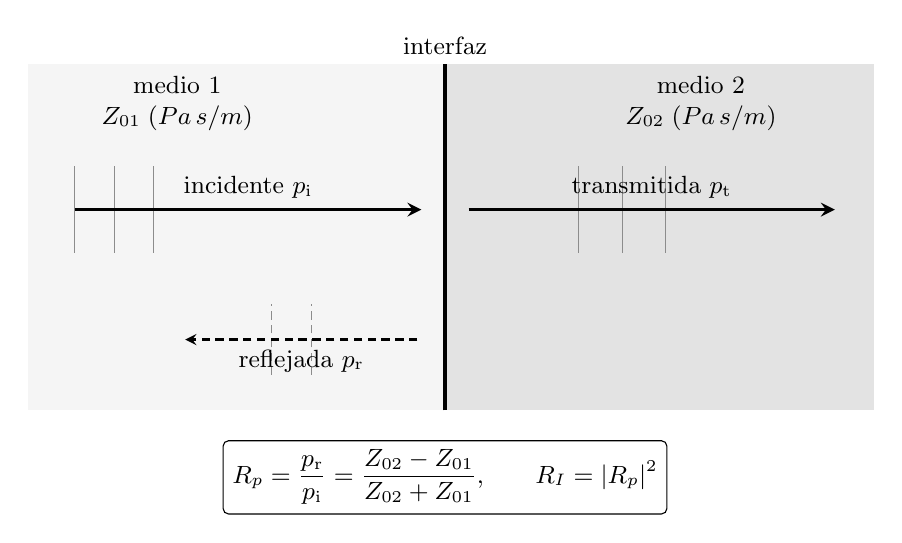
\begin{tikzpicture}[font=\small,>=stealth,x=1cm,y=1cm]
    \fill[black!4] (0.45,0.75) rectangle (5.75,5.15);
    \fill[black!11] (5.75,0.75) rectangle (11.20,5.15);
    \draw[very thick] (5.75,0.75) -- (5.75,5.15);
    \node[above] at (5.75,5.15) {interfaz};

    \node[align=center] at (2.35,4.65)
        {medio 1\\\(Z_{01}\;(\text{Pa}\,\text{s}/\text{m})\)};
    \node[align=center] at (9.00,4.65)
        {medio 2\\\(Z_{02}\;(\text{Pa}\,\text{s}/\text{m})\)};

    \foreach \x in {1.05,1.55,2.05}{
        \draw[black!45] (\x,2.75) -- (\x,3.85);
    }
    \foreach \x in {3.55,4.05}{
        \draw[black!45,densely dashed] (\x,1.20) -- (\x,2.10);
    }
    \foreach \x in {7.45,8.00,8.55}{
        \draw[black!45] (\x,2.75) -- (\x,3.85);
    }

    \draw[->,very thick] (1.05,3.30) -- (5.45,3.30)
        node[midway,above] {incidente \(p_\mathrm{i}\)};
    \draw[->,thick,densely dashed] (5.40,1.65) -- (2.45,1.65)
        node[midway,below] {reflejada \(p_\mathrm{r}\)};
    \draw[->,very thick] (6.05,3.30) -- (10.70,3.30)
        node[midway,above] {transmitida \(p_\mathrm{t}\)};

    \node[draw,rounded corners=2pt,fill=white,align=center] at (5.75,-0.10)
        {\(\displaystyle R_p=\frac{p_\mathrm{r}}{p_\mathrm{i}}
          =\frac{Z_{02}-Z_{01}}{Z_{02}+Z_{01}}\),\qquad
          \(\displaystyle R_I=|R_p|^2\)};
\end{tikzpicture}

    \caption{Incidencia normal sobre una interfaz ideal. La onda incidente se
    separa en una componente reflejada y otra transmitida; el coeficiente
    \(R_p\) depende de las impedancias \(Z_{01}\) y \(Z_{02}\), y
    \(R_I=|R_p|^2\) expresa la fracción de intensidad reflejada bajo las
    hipótesis indicadas en el texto. Elaboración propia a partir de la
    ecuación~\eqref{eq:u4-reflexion-presion}.}
    \label{fig:u4-impedancia-reflexion}
\end{figure}

\subsection{Intensidad, potencia y energía}
\label{sec:u4-intensidad-potencia}

En una descripción unidimensional, la \textbf{intensidad acústica instantánea}
\(i(t)\) es el producto de la presión acústica \(p(t)\), medida en pascales, y
la velocidad de partícula \(u(t)\), medida en metros por segundo:

\begin{equation}
    i(t)=p(t)u(t).
    \label{eq:u4-intensidad-instantanea}
\end{equation}

La unidad de \(i(t)\) es el watt por metro cuadrado
(\(\text{W}/\text{m}^2\)). El signo instantáneo indica el sentido del flujo de
energía respecto de la dirección elegida.

Para un intervalo de observación de duración \(\Delta t\), medido en segundos,
se definirá la \textbf{intensidad acústica media} \(I\), en
\(\text{W}/\text{m}^2\), mediante

\begin{equation}
    I=\frac{1}{\Delta t}
      \int_{t_0}^{t_0+\Delta t}p(t)u(t)\,\mathrm{d}t,
    \label{eq:u4-intensidad-media}
\end{equation}

donde \(t_0\) es el instante inicial del promedio. Para una señal periódica,
\(\Delta t\) suele elegirse como un número entero de períodos.

En una onda plana progresiva sinusoidal, en un fluido sin pérdidas, la
intensidad media también puede calcularse mediante~\cite{xiangBlauert2021}

\begin{equation}
    I=p_\mathrm{rms}u_\mathrm{rms}
     =\frac{p_\mathrm{rms}^2}{Z_0}
     =Z_0u_\mathrm{rms}^2,
    \label{eq:u4-intensidad-onda-plana}
\end{equation}

donde \(p_\mathrm{rms}\) es la presión eficaz en pascales y
\(u_\mathrm{rms}\) la velocidad eficaz en metros por segundo.

La \textbf{potencia acústica} \(W\) es la energía acústica transferida por
unidad de tiempo y se mide en watts (\(\text{W}\)). Si una superficie \(S\),
medida en metros cuadrados (\(\text{m}^2\)), recibe una intensidad uniforme y
normal a ella, entonces

\begin{equation}
    W=IS.
    \label{eq:u4-potencia-uniforme}
\end{equation}

En el caso general se debe sumar el flujo de intensidad a través de toda la
superficie. Si una potencia constante \(W\) actúa durante un intervalo
\(\Delta t\), la energía transferida \(E_\mathrm{ac}\), medida en joules
(\(\text{J}\)), es

\begin{equation}
    E_\mathrm{ac}=W\Delta t.
    \label{eq:u4-energia-acustica}
\end{equation}

\subsection{Ejemplo resuelto: presión, velocidad e intensidad}
\label{sec:u4-ejemplo-magnitudes}

Se considera, como dato de un modelo de onda plana progresiva, una presión
eficaz \(p_\mathrm{rms}=0{,}20\,\text{Pa}\) y una impedancia característica
\(Z_0=400\,\text{Pa}\,\text{s}/\text{m}\). Estos valores son datos
didácticos y no describen una medición clínica.

La velocidad eficaz de partícula es

\[
    u_\mathrm{rms}
      =\frac{p_\mathrm{rms}}{Z_0}
      =\frac{0{,}20\,\text{Pa}}
             {400\,\text{Pa}\,\text{s}/\text{m}}
      =5{,}0\times10^{-4}\,\text{m}/\text{s}.
\]

La intensidad media es

\[
    I=\frac{p_\mathrm{rms}^2}{Z_0}
      =\frac{(0{,}20\,\text{Pa})^2}
             {400\,\text{Pa}\,\text{s}/\text{m}}
      =1{,}0\times10^{-4}\,\text{W}/\text{m}^2.
\]

El ejemplo muestra que presión, velocidad e intensidad tienen unidades
diferentes. La igualdad numérica entre dos resultados en otro problema no
volvería equivalentes a las magnitudes.

La figura~\ref{fig:u4-presion-velocidad-intensidad} representa un período
normalizado. Separar las tres curvas permite observar que la intensidad
instantánea no es otra amplitud de la sinusoide: es el producto \(p(t)u(t)\).

\begin{figure}[!htbp]
    \centering
    % Propósito: mostrar que presión y velocidad de partícula están en fase en una
% onda plana progresiva, mientras la intensidad instantánea es su producto.
% Origen: p=p_hat sin(omega t), u=u_hat sin(omega t) e
% i=p_hat u_hat sin^2(omega t), bajo las hipótesis de la
% ecuación \eqref{eq:u4-impedancia-caracteristica}.
% Curvas teóricas normalizadas; no representan datos medidos.
% Descripción accesible: tres gráficos comparten un período. La presión y la
% velocidad normalizadas tienen la misma forma sinusoidal y cruzan cero a la
% vez. La intensidad normalizada es siempre no negativa y presenta dos máximos
% por período, lo que indica flujo neto de energía en la dirección de avance.
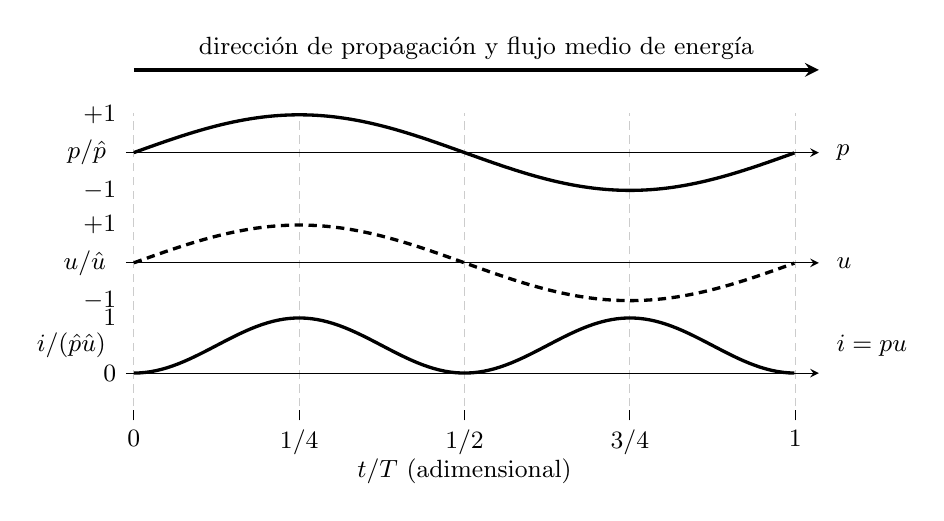
\begin{tikzpicture}[font=\small,>=stealth,x=1cm,y=1cm]
    \draw[->,very thick] (2.15,4.20) -- (10.85,4.20)
        node[midway,above] {dirección de propagación y flujo medio de energía};

    \foreach \q/\lab in {0/{0},0.25/{1/4},0.5/{1/2},0.75/{3/4},1/{1}}{
        \pgfmathsetmacro{\xx}{2.15+8.4*\q}
        \draw[densely dashed,black!20] (\xx,-0.25) -- (\xx,3.65);
        \draw (\xx,-0.25) -- (\xx,-0.12);
        \node[below] at (\xx,-0.25) {\(\lab\)};
    }

    \foreach \yy in {3.15,1.75,0.35}{
        \draw[->] (2.05,\yy) -- (10.85,\yy);
    }

    \node[anchor=east] at (1.92,3.15) {\(p/\hat p\)};
    \node[anchor=east] at (1.92,1.75) {\(u/\hat u\)};
    \node[anchor=east,align=right] at (1.92,0.70)
        {\(i/(\hat p\hat u)\)};

    \node[anchor=east] at (2.05,3.63) {\(+1\)};
    \node[anchor=east] at (2.05,2.67) {\(-1\)};
    \node[anchor=east] at (2.05,2.23) {\(+1\)};
    \node[anchor=east] at (2.05,1.27) {\(-1\)};
    \node[anchor=east] at (2.05,1.05) {\(1\)};
    \node[anchor=east] at (2.05,0.35) {\(0\)};

    \draw[very thick,samples=120,domain=0:1]
        plot ({2.15+8.4*\x},{3.15+0.48*sin(360*\x)});
    \draw[very thick,densely dashed,samples=120,domain=0:1]
        plot ({2.15+8.4*\x},{1.75+0.48*sin(360*\x)});
    \draw[very thick,samples=120,domain=0:1]
        plot ({2.15+8.4*\x},{0.35+0.70*(sin(360*\x))^2});

    \node[anchor=west] at (10.95,3.15) {\(p\)};
    \node[anchor=west] at (10.95,1.75) {\(u\)};
    \node[anchor=west] at (10.95,0.70) {\(i=pu\)};
    \node at (6.35,-0.90) {\(t/T\) (adimensional)};
\end{tikzpicture}

    \caption{Presión, velocidad de partícula e intensidad instantánea
    normalizadas para una onda plana progresiva sinusoidal. Presión y velocidad
    están en fase; su producto es no negativo y representa flujo de energía en
    la dirección de propagación. Las curvas son teóricas y adimensionales.
    Elaboración propia a partir de las
    ecuaciones~\eqref{eq:u4-impedancia-caracteristica}
    y~\eqref{eq:u4-intensidad-instantanea}.}
    \label{fig:u4-presion-velocidad-intensidad}
\end{figure}

\section{Valores de una señal acústica}
\label{sec:u4-valores-senal}

Una señal variable no queda descrita por un único número. Antes de comparar
mediciones se debe indicar qué valor se informa y durante qué intervalo se
calculó.

Para una presión \(p(t)\), medida en pascales, se distinguen:

\begin{description}[style=nextline]
    \item[\textbf{Valor instantáneo:}]
    el valor de \(p(t)\) en un instante particular.

    \item[\textbf{Amplitud de pico:}]
    el máximo valor absoluto respecto del equilibrio. Se representará mediante
    \(\hat p\) y se medirá en pascales.

    \item[\textbf{Valor pico a pico:}]
    la diferencia \(p_\mathrm{pp}=p_{\max}-p_{\min}\), medida en pascales.
    Para una sinusoide centrada en cero, \(p_\mathrm{pp}=2\hat p\).

    \item[\textbf{Valor medio:}]
    el promedio algebraico durante un intervalo \(\Delta t\):
\end{description}

\begin{equation}
    \overline p
      =\frac{1}{\Delta t}
       \int_{t_0}^{t_0+\Delta t}p(t)\,\mathrm{d}t.
    \label{eq:u4-presion-media}
\end{equation}

El valor medio de una sinusoide centrada en cero, calculado sobre un número
entero de períodos, es cero. Esto no significa que la señal no produzca
transferencia de energía.

El \textbf{valor eficaz} o RMS de la presión se representará mediante
\(p_\mathrm{rms}\), se medirá en pascales y se definirá como

\begin{equation}
    p_\mathrm{rms}
      =\sqrt{\frac{1}{\Delta t}
       \int_{t_0}^{t_0+\Delta t}p^2(t)\,\mathrm{d}t}.
    \label{eq:u4-presion-rms}
\end{equation}

Elevar al cuadrado evita que las partes positivas y negativas se cancelen.
Después de promediar, la raíz devuelve la unidad original de presión.

Para una presión sinusoidal de media nula,

\begin{equation}
    p(t)=\hat p\sin(2\pi ft+\varphi),
    \label{eq:u4-presion-sinusoidal}
\end{equation}

donde \(f\) es la frecuencia en hertz y \(\varphi\) la fase inicial en
radianes, se obtiene

\begin{equation}
    p_\mathrm{rms}=\frac{\hat p}{\sqrt{2}}.
    \label{eq:u4-rms-sinusoide}
\end{equation}

\subsection{Ejemplo resuelto: pico y valor eficaz}
\label{sec:u4-ejemplo-rms}

Una presión sinusoidal posee una amplitud de pico
\(\hat p=0{,}283\,\text{Pa}\). Su valor pico a pico es

\[
    p_\mathrm{pp}=2\hat p=0{,}566\,\text{Pa},
\]

y su valor eficaz es

\[
    p_\mathrm{rms}
      =\frac{0{,}283\,\text{Pa}}{\sqrt{2}}
      \approx0{,}200\,\text{Pa}.
\]

El valor medio sobre un número entero de períodos es cero. Pico, pico a pico,
media y RMS describen aspectos diferentes de la misma señal.

La figura~\ref{fig:u4-rms-sinusoide} muestra por qué el valor medio de
\(p(t)\) y el RMS responden preguntas diferentes. La presión cambia de signo,
pero su cuadrado no; por eso el promedio de \(p^2(t)\) conserva información
sobre el tamaño de la variación.

\begin{figure}[!htbp]
    \centering
    % Propósito: hacer visible la secuencia cuadrado-promedio-raíz que define el
% RMS y diferenciarla del valor medio de la presión.
% Origen: p/p_hat=sin(2 pi t/T),
% overline{p}=0, overline{p^2}/p_hat^2=1/2 y
% p_rms/p_hat=1/sqrt(2), ecuaciones \eqref{eq:u4-presion-media},
% \eqref{eq:u4-presion-rms} y \eqref{eq:u4-rms-sinusoide}.
% Curvas teóricas normalizadas; no representan datos medidos.
% Descripción accesible: el panel superior muestra una sinusoide con media
% cero y picos positivos y negativos. El panel inferior muestra su cuadrado,
% siempre no negativo, cuya media normalizada es un medio. Al tomar la raíz
% de esa media se obtiene un RMS igual al pico dividido por raíz de dos.
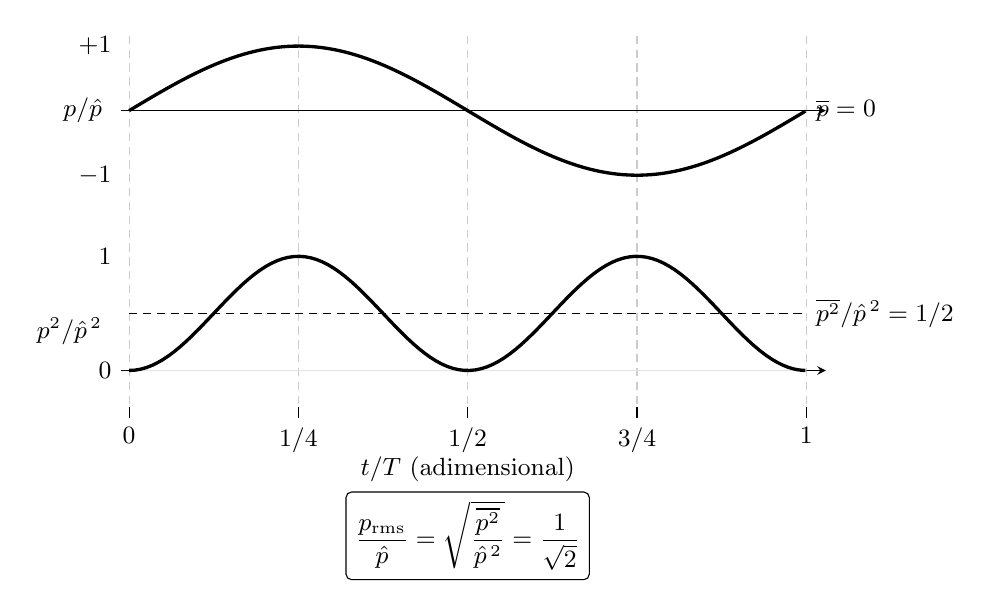
\begin{tikzpicture}[font=\small,>=stealth,x=1cm,y=1cm]
    \foreach \q/\lab in {0/{0},0.25/{1/4},0.5/{1/2},0.75/{3/4},1/{1}}{
        \pgfmathsetmacro{\xx}{2.10+8.6*\q}
        \draw[densely dashed,black!20] (\xx,-1.05) -- (\xx,3.85);
        \draw (\xx,-1.05) -- (\xx,-0.92);
        \node[below] at (\xx,-1.05) {\(\lab\)};
    }

    \draw[->] (2.00,2.85) -- (10.95,2.85);
    \draw[->] (2.00,-0.45) -- (10.95,-0.45);
    \node[anchor=east] at (1.88,2.85) {\(p/\hat p\)};
    \node[anchor=east,align=right] at (1.88,0.05)
        {\(p^2/\hat p^{\,2}\)};

    \draw[very thick,samples=120,domain=0:1]
        plot ({2.10+8.6*\x},{2.85+0.82*sin(360*\x)});
    \draw[densely dashed] (2.10,2.85) -- (10.70,2.85)
        node[anchor=west] {\(\overline p=0\)};
    \node[anchor=east] at (2.00,3.67) {\(+1\)};
    \node[anchor=east] at (2.00,2.03) {\(-1\)};

    \draw[black!10] (2.10,-0.45)
        plot[samples=120,domain=0:1]
        ({2.10+8.6*\x},{-0.45+1.45*(sin(360*\x))^2})
        -- (10.70,-0.45) -- cycle;
    \draw[very thick,samples=120,domain=0:1]
        plot ({2.10+8.6*\x},{-0.45+1.45*(sin(360*\x))^2});
    \draw[densely dashed] (2.10,0.275) -- (10.70,0.275)
        node[anchor=west] {\(\overline{p^2}/\hat p^{\,2}=1/2\)};
    \node[anchor=east] at (2.00,1.00) {\(1\)};
    \node[anchor=east] at (2.00,-0.45) {\(0\)};

    \node at (6.40,-1.70) {\(t/T\) (adimensional)};
    \node[draw,rounded corners=2pt,fill=white] at (6.40,-2.55)
        {\(\displaystyle
          \frac{p_\mathrm{rms}}{\hat p}
          =\sqrt{\frac{\overline{p^2}}{\hat p^{\,2}}}
          =\frac{1}{\sqrt{2}}\)};
\end{tikzpicture}

    \caption{Construcción del valor eficaz de una presión sinusoidal durante
    un período. La presión normalizada tiene media cero, mientras que su
    cuadrado posee media \(1/2\); al tomar la raíz se obtiene
    \(p_\mathrm{rms}/\hat p=1/\sqrt{2}\). Curvas teóricas normalizadas.
    Elaboración propia a partir de las
    ecuaciones~\eqref{eq:u4-presion-media}
    y~\eqref{eq:u4-presion-rms}.}
    \label{fig:u4-rms-sinusoide}
\end{figure}

\subsection{Tono puro y señales complejas}
\label{sec:u4-tono-complejo}

La Unidad~\ref{chap:unidad-3} definió el tono puro ideal como una señal
sinusoidal. Una \textbf{señal compleja} es, en este contexto, una señal cuya
forma temporal no es una única sinusoide. Puede contener componentes
periódicas, aperiódicas y transitorias.

La representación mediante componentes frecuenciales, la distinción entre
fundamental, armónicos y parciales, y el análisis de la voz corresponden al
capítulo siguiente. Aquí interesa que las definiciones de media y RMS se
aplican también a señales no sinusoidales, mientras que
\(p_\mathrm{rms}=\hat p/\sqrt{2}\) no puede usarse automáticamente para
cualquier forma de señal.

\section{Niveles logarítmicos}
\label{sec:u4-niveles}

El decibel, de símbolo \(\text{dB}\), expresa una relación logarítmica. Un
valor en decibeles solo puede interpretarse si se conoce:

\begin{enumerate}
    \item la magnitud comparada;
    \item el valor de referencia;
    \item cualquier ponderación o condición adicional.
\end{enumerate}

\subsection{Nivel de presión sonora}
\label{sec:u4-nivel-presion}

Se representará el nivel de presión sonora mediante \(L_p\). Para una presión
eficaz \(p_\mathrm{rms}\) y una presión de referencia
\(p_\mathrm{ref}\), ambas en pascales, se define

\begin{equation}
    L_p=20\log_{10}\!\left(
        \frac{p_\mathrm{rms}}{p_\mathrm{ref}}\right).
    \label{eq:u4-nivel-presion}
\end{equation}

El cociente dentro del logaritmo es adimensional. Para sonidos en aire
se utiliza habitualmente \(p_\mathrm{ref}=20\,\mu\text{Pa}\); cuando esta
referencia está implícita, el resultado se expresa como nivel de presión
sonora en \(\text{dB SPL}\)~\cite{nistSP811,iso1683_2015}.

En acústica subacuática se utiliza una referencia de presión diferente,
habitualmente \(1\,\mu\text{Pa}\), que debe declararse de forma explícita~\cite{nistSP811,iso1683_2015}.
Dos niveles con referencias distintas no pueden compararse como si
describieran la misma razón.

La figura~\ref{fig:u4-escala-presion-db-spl} presenta la correspondencia
matemática para la referencia de aire. Cada multiplicación de la presión
eficaz por diez agrega \(20\,\text{dB}\). La escala no representa sonoridad,
umbrales auditivos ni una referencia válida para otro medio.

\begin{figure}[htbp]
    \centering
    % Propósito: vincular una escala logarítmica de nivel con las presiones
% eficaces correspondientes y mostrar que multiplicar la presión por diez
% agrega 20 dB.
% Origen: L_p=20 log10(p_rms/p_ref), con p_ref=20 microPa,
% ecuación \eqref{eq:u4-nivel-presion}. Los valores son resultados exactos de
% la relación matemática, no umbrales perceptuales ni datos medidos.
% Descripción accesible: una escala horizontal presenta niveles desde 0 hasta
% 120 dB SPL en pasos de 20 dB. Debajo de cada nivel aparece la presión eficaz
% correspondiente, desde 20 micropascales hasta 20 pascales. Cada paso
% multiplica la presión por diez.
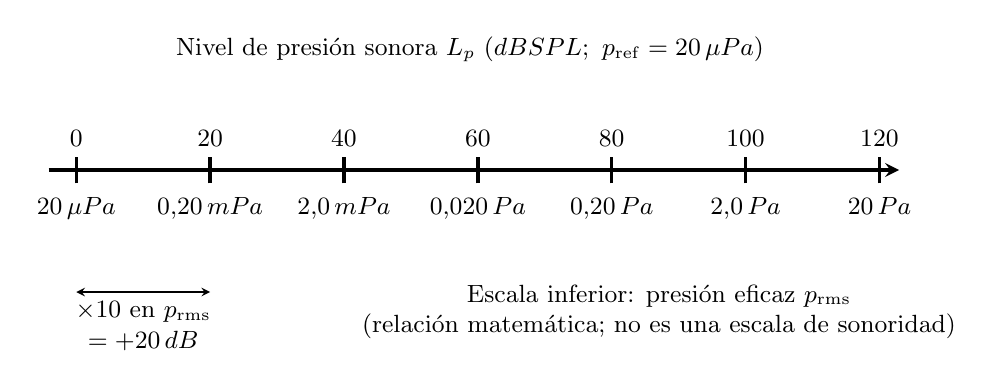
\begin{tikzpicture}[font=\small,>=stealth,x=1cm,y=1cm]
    \draw[->,very thick] (0.75,2.15) -- (11.55,2.15);
    \node[above,align=center] at (6.10,3.40)
        {Nivel de presión sonora \(L_p\)
        \((\text{dB SPL};\ p_\mathrm{ref}=20\,\mu\text{Pa})\)};

    \foreach \x/\lev/\press in {
        1.10/0/{20\,\mu\text{Pa}},
        2.80/20/{0{,}20\,\text{mPa}},
        4.50/40/{2{,}0\,\text{mPa}},
        6.20/60/{0{,}020\,\text{Pa}},
        7.90/80/{0{,}20\,\text{Pa}},
        9.60/100/{2{,}0\,\text{Pa}},
        11.30/120/{20\,\text{Pa}}}{
        \draw[very thick] (\x,1.98) -- (\x,2.32);
        \node[above] at (\x,2.32) {\(\lev\)};
        \node[below,align=center] at (\x,1.93) {\(\press\)};
    }

    \draw[<->] (1.10,0.60) -- (2.80,0.60)
        node[midway,below,align=center]
        {\(\times10\) en \(p_\mathrm{rms}\)\\\(=+20\,\text{dB}\)};
    \node[align=center] at (8.50,0.35)
        {Escala inferior: presión eficaz \(p_\mathrm{rms}\)\\
        (relación matemática; no es una escala de sonoridad)};
\end{tikzpicture}

    \caption{Correspondencia entre presión eficaz y nivel de presión sonora
    para \(p_\mathrm{ref}=20\,\mu\text{Pa}\). Los valores proceden únicamente
    de \(L_p=20\log_{10}(p_\mathrm{rms}/p_\mathrm{ref})\): no son datos
    experimentales ni una escala perceptual. Elaboración propia a partir de la
    ecuación~\eqref{eq:u4-nivel-presion}.}
    \label{fig:u4-escala-presion-db-spl}
\end{figure}

\subsection{Niveles de intensidad y potencia}
\label{sec:u4-niveles-energia}

Se representará el nivel de intensidad mediante \(L_I\). Para una intensidad
media \(I\), en \(\text{W}/\text{m}^2\), y una intensidad de referencia
\(I_\mathrm{ref}\), en la misma unidad, se define

\begin{equation}
    L_I=10\log_{10}\!\left(\frac{I}{I_\mathrm{ref}}\right).
    \label{eq:u4-nivel-intensidad}
\end{equation}

Se representará el nivel de potencia mediante \(L_W\). Para una potencia
acústica \(W\), en watts, y una potencia de referencia \(W_\mathrm{ref}\), en
watts, se define
\nopagebreak[4]

\begin{equation}
    L_W=10\log_{10}\!\left(\frac{W}{W_\mathrm{ref}}\right).
    \label{eq:u4-nivel-potencia}
\end{equation}

En acústica aérea se emplean comúnmente
\(I_\mathrm{ref}=10^{-12}\,\text{W}/\text{m}^2\) y
\(W_\mathrm{ref}=10^{-12}\,\text{W}\)~\cite{nistSP811,iso1683_2015}. La referencia debe acompañar cualquier
uso que pueda resultar ambiguo.

\subsection{Por qué aparecen 10 y 20}
\label{sec:u4-factores-logaritmicos}

Intensidad y potencia son magnitudes asociadas directamente con una tasa de
transferencia de energía; por eso sus niveles usan el factor \(10\). En la
onda plana progresiva de la ecuación~\eqref{eq:u4-intensidad-onda-plana}, y si
la impedancia no cambia, la intensidad es proporcional al cuadrado de la
presión eficaz. Entonces

\[
    10\log_{10}\!\left[
       \left(\frac{p_\mathrm{rms}}{p_\mathrm{ref}}\right)^2
    \right]
    =20\log_{10}\!\left(
       \frac{p_\mathrm{rms}}{p_\mathrm{ref}}\right).
\]

El factor \(20\) no convierte la presión en intensidad: aparece porque el
nivel de una magnitud cuadrática se expresó mediante una razón de amplitudes.

\subsection{Ejemplo resuelto: presión y dB SPL}
\label{sec:u4-ejemplo-nivel}

Una medición en aire informa
\(p_\mathrm{rms}=0{,}20\,\text{Pa}\). Con
\(p_\mathrm{ref}=20\,\mu\text{Pa}
=2{,}0\times10^{-5}\,\text{Pa}\), el nivel es

\[
    L_p
      =20\log_{10}\!\left(
       \frac{0{,}20}{2{,}0\times10^{-5}}\right)
      =20\log_{10}(10^4)
      =80\,\text{dB SPL}.
\]

Este resultado es un nivel físico de presión. No especifica por sí solo una
sonoridad ni un nivel audiométrico.

\subsection{Niveles físicos y escalas auditivas}
\label{sec:u4-niveles-auditivos}

El nivel de audición expresado en \(\text{dB HL}\) depende de
referencias audiométricas vinculadas con la frecuencia y el transductor. No
debe convertirse directamente a \(\text{dB SPL}\) sin los datos de calibración
correspondientes~\cite{iso389_1_2017}.

Las ponderaciones frecuenciales, como A, C y Z, se aplican en
mediciones electroacústicas con objetivos definidos y no son nombres
alternativos para \(\text{dB SPL}\) o \(\text{dB HL}\)~\cite{iec61672_1_2013}. Su desarrollo se
reserva para el capítulo de análisis frecuencial y sonometría.

\section{Superposición, coherencia y suma de niveles}
\label{sec:u4-coherencia-suma}

El principio de superposición de la Unidad~\ref{chap:unidad-3} establece que,
en un sistema lineal, las presiones acústicas instantáneas presentes en un
mismo punto se suman algebraicamente:
\nopagebreak[4]

\begin{equation}
    p_\mathrm{R}(t)=p_1(t)+p_2(t).
    \label{eq:u4-suma-presiones}
\end{equation}

El resultado en RMS o en decibeles depende de la relación temporal entre las
señales.

\subsection{Fuentes coherentes}
\label{sec:u4-fuentes-coherentes}

Dos señales sinusoidales de la misma frecuencia son coherentes cuando mantienen
una diferencia de fase constante. Si sus presiones eficaces son
\(p_{1,\mathrm{rms}}\) y \(p_{2,\mathrm{rms}}\), ambas en pascales, y su
diferencia de fase es \(\Delta\varphi\), en radianes, la presión eficaz
resultante satisface

\begin{equation}
    p_{\mathrm{R,rms}}^2
      =p_{1,\mathrm{rms}}^2+p_{2,\mathrm{rms}}^2
       +2p_{1,\mathrm{rms}}p_{2,\mathrm{rms}}
        \cos(\Delta\varphi).
    \label{eq:u4-suma-coherente}
\end{equation}

Para presiones iguales y en fase, la presión se duplica y el nivel aumenta

\[
    20\log_{10}(2)\approx6{,}02\,\text{dB}.
\]

Este aumento no corresponde a cualquier par de fuentes coherentes. Con otros
desfases puede producirse un aumento menor, una reducción o, en el caso ideal
de igual amplitud y oposición de fase, una cancelación en el punto considerado.

\subsection{Señales no correlacionadas}
\label{sec:u4-fuentes-no-correlacionadas}

Cuando dos presiones no están correlacionadas durante el intervalo de
observación, el término cruzado medio es nulo y se suman sus cuadrados
eficaces:

\begin{equation}
    p_{\mathrm{R,rms}}^2
      =p_{1,\mathrm{rms}}^2+p_{2,\mathrm{rms}}^2.
    \label{eq:u4-suma-no-correlacionada}
\end{equation}

Si \(L_1\) y \(L_2\) son niveles de presión sonora expresados con la misma
referencia, el nivel total es

\begin{equation}
    L_\mathrm{R}
      =10\log_{10}\!\left(
        10^{L_1/10}+10^{L_2/10}\right).
    \label{eq:u4-suma-niveles}
\end{equation}

Para dos niveles iguales de \(70\,\text{dB SPL}\),

\[
    L_\mathrm{R}
      =10\log_{10}\!\left(
        2\times10^{70/10}\right)
      =70+10\log_{10}(2)
      \approx73{,}01\,\text{dB SPL}.
\]

El aumento de \(3{,}01\,\text{dB}\) corresponde a señales no correlacionadas
de igual nivel, no a la suma de dos valores numéricos de \(70\,\text{dB}\).

La figura~\ref{fig:u4-suma-coherente-no-correlacionada} compara los dos casos
para señales de igual presión eficaz. La diferencia entre \(6{,}02\,\text{dB}\)
y \(3{,}01\,\text{dB}\) no se debe a una regla distinta del decibel, sino a
qué cantidades pueden sumarse bajo cada relación temporal.

\begin{figure}[htbp]
    \centering
    % Propósito: distinguir la suma instantánea de presiones coherentes de la suma
% de cuadrados eficaces para señales no correlacionadas.
% Origen: ecuaciones \eqref{eq:u4-suma-coherente} y
% \eqref{eq:u4-suma-no-correlacionada}, para dos señales de igual
% p_rms. Los incrementos son 20 log10(2)=6,02 dB y
% 10 log10(2)=3,01 dB.
% Esquema matemático; no representa mediciones ni fuentes particulares.
% Descripción accesible: el panel izquierdo muestra dos presiones coherentes
% iguales y en fase, que se suman hasta duplicar la presión y aumentar el nivel
% 6,02 dB. El derecho muestra dos presiones iguales no correlacionadas, cuyos
% cuadrados eficaces se suman; el RMS crece por raíz de dos y el nivel 3,01 dB.
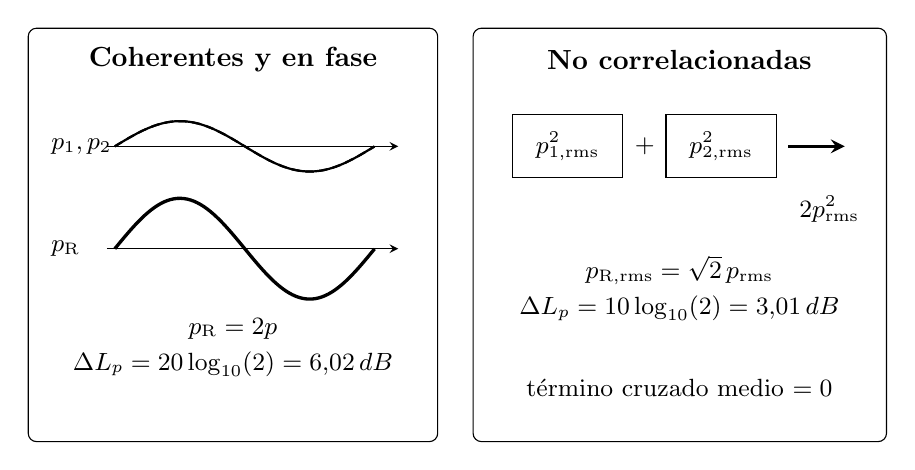
\begin{tikzpicture}[font=\small,>=stealth,x=1cm,y=1cm]
    \draw[rounded corners=3pt] (0.35,0.10) rectangle (5.55,5.35);
    \draw[rounded corners=3pt] (6.00,0.10) rectangle (11.25,5.35);

    \node[font=\bfseries] at (2.95,4.95) {Coherentes y en fase};
    \node[font=\bfseries] at (8.62,4.95) {No correlacionadas};

    \draw[->] (1.35,3.85) -- (5.05,3.85);
    \draw[thick,samples=80,domain=0:1]
        plot ({1.45+3.30*\x},{3.85+0.32*sin(360*\x)});
    \draw[thick,densely dashed,samples=80,domain=0:1]
        plot ({1.45+3.30*\x},{3.85+0.32*sin(360*\x)});
    \node[anchor=west] at (0.52,3.85) {\(p_1,p_2\)};

    \draw[->] (1.35,2.55) -- (5.05,2.55);
    \draw[very thick,samples=80,domain=0:1]
        plot ({1.45+3.30*\x},{2.55+0.64*sin(360*\x)});
    \node[anchor=west] at (0.52,2.55) {\(p_\mathrm{R}\)};

    \node[align=center] at (2.95,1.30)
        {\(p_\mathrm{R}=2p\)\\[2pt]
         \(\Delta L_p=20\log_{10}(2)=6{,}02\,\text{dB}\)};

    \node[draw,minimum width=1.40cm,minimum height=0.80cm] at (7.20,3.85)
        {\(p_{1,\mathrm{rms}}^2\)};
    \node at (8.18,3.85) {\(+\)};
    \node[draw,minimum width=1.40cm,minimum height=0.80cm] at (9.15,3.85)
        {\(p_{2,\mathrm{rms}}^2\)};
    \draw[->,very thick] (10.00,3.85) -- (10.72,3.85);
    \node[anchor=west,align=left] at (10.02,3.05)
        {\(2p_\mathrm{rms}^2\)};

    \node[align=center] at (8.62,2.05)
        {\(p_{\mathrm{R,rms}}=\sqrt{2}\,p_\mathrm{rms}\)\\[2pt]
         \(\Delta L_p=10\log_{10}(2)=3{,}01\,\text{dB}\)};
    \node[align=center] at (8.62,0.78)
        {término cruzado medio \(=0\)};
\end{tikzpicture}

    \caption{Suma de dos señales de igual presión eficaz. Si son coherentes y
    llegan en fase, la presión se duplica y el nivel aumenta
    \(6{,}02\,\text{dB}\). Si no están correlacionadas, se suman los cuadrados
    eficaces y el aumento es \(3{,}01\,\text{dB}\). Esquema matemático, no
    medición. Elaboración propia a partir de las
    ecuaciones~\eqref{eq:u4-suma-coherente}
    y~\eqref{eq:u4-suma-no-correlacionada}.}
    \label{fig:u4-suma-coherente-no-correlacionada}
\end{figure}

\subsection{Correlación parcial}
\label{sec:u4-correlacion-parcial}

Entre los casos completamente coherente y no correlacionado pueden existir
grados intermedios de correlación. Se representará mediante \(\gamma\) un
coeficiente de correlación normalizado, adimensional, comprendido entre
\(-1\) y \(1\). Para dos señales dentro del mismo intervalo de promedio,

\begin{equation}
    p_{\mathrm{R,rms}}^2
      =p_{1,\mathrm{rms}}^2+p_{2,\mathrm{rms}}^2
       +2\gamma p_{1,\mathrm{rms}}p_{2,\mathrm{rms}}.
    \label{eq:u4-suma-correlacion-parcial}
\end{equation}

El valor \(\gamma=0\) reproduce la suma no correlacionada. Para dos sinusoides
coherentes del mismo período de promedio,
\(\gamma=\cos(\Delta\varphi)\). La correlación no es una propiedad de la
fuente por su nombre: debe referirse a las señales observadas, al punto de
medición y al intervalo considerado.

\section{Geometría del campo acústico}
\label{sec:u4-geometria-campo}

La geometría de los frentes de onda permite construir modelos de propagación.
Son idealizaciones: una fuente real puede aproximarse a uno u otro modelo solo
en determinadas regiones y bandas de frecuencia.

\begin{description}[style=nextline]
    \item[\textbf{Onda plana:}]
    los frentes de igual fase se aproximan mediante planos paralelos. En un
    medio sin pérdidas no existe dispersión geométrica porque el área del
    frente considerada permanece constante.

    \item[\textbf{Onda cilíndrica:}]
    los frentes se aproximan mediante cilindros coaxiales. Para una fuente
    lineal ideal y suficientemente extensa, el área lateral por unidad de
    longitud es proporcional a la distancia radial \(r\). En ausencia de
    pérdidas, \(I\propto1/r\), de modo que el nivel disminuye aproximadamente
    \(3{,}01\,\text{dB}\) al duplicar \(r\).

    \item[\textbf{Onda esférica:}]
    los frentes se aproximan mediante esferas concéntricas. Para una fuente
    puntual ideal, el área es proporcional a \(r^2\), de modo que
    \(I\propto1/r^2\).
\end{description}

Una onda dentro de un tubo uniforme no debe llamarse cilíndrica solo porque el
tubo tenga sección circular. Por debajo de determinadas frecuencias, el modo
dominante de un conducto puede aproximarse mediante una onda plana. La
respuesta acústica del conducto auditivo externo requiere además considerar su
geometría, terminación y resonancias, temas que se abordarán junto con el
sistema auditivo.

\subsection{Campo libre, campo reverberante y campo difuso}
\label{sec:u4-tipos-campo}

Un \textbf{campo libre} es un modelo en el que las reflexiones de los límites
son despreciables en la región de interés. No es sinónimo de cualquier recinto
con superficies absorbentes.

Un \textbf{campo reverberante} contiene una contribución significativa de
reflexiones sucesivas. No toda reflexión se percibe como un eco separado.

Un campo difuso ideal presenta, en promedio, flujo de energía
distribuido en todas las direcciones y propiedades estadísticas
aproximadamente uniformes en la región considerada~\cite{xiangBlauert2021}. Una sala ruidosa no es
necesariamente un campo difuso.

La audiometría en campo sonoro requiere condiciones geométricas,
electroacústicas y de calibración específicas; puede utilizar campos libre,
cuasilibre o difuso según el procedimiento adoptado~\cite{iso8253_2_2009}. El diseño y la
verificación de recintos se desarrollarán en el capítulo dedicado a
propagación, aislamiento y cabinas.

\section{Ley del cuadrado inverso}
\label{sec:u4-cuadrado-inverso}

Se considera una fuente puntual omnidireccional ideal que emite una potencia
acústica constante \(W\), medida en watts, en un medio homogéneo y sin pérdidas.
En campo libre, esa potencia atraviesa una esfera de radio \(r\), medido en
metros, cuya superficie es \(4\pi r^2\). La intensidad media \(I(r)\), medida
en \(\text{W}/\text{m}^2\), es

\begin{equation}
    I(r)=\frac{W}{4\pi r^2}.
    \label{eq:u4-cuadrado-inverso}
\end{equation}

Para dos distancias \(r_1\) y \(r_2\),

\begin{equation}
    \frac{I_2}{I_1}
      =\left(\frac{r_1}{r_2}\right)^2.
    \label{eq:u4-razon-intensidades-distancia}
\end{equation}

La diferencia de nivel de intensidad es, por lo tanto,

\begin{equation}
    L_{I2}-L_{I1}
      =-20\log_{10}\!\left(\frac{r_2}{r_1}\right).
    \label{eq:u4-nivel-intensidad-distancia}
\end{equation}

En la región de campo lejano de una onda esférica progresiva, y si la
impedancia del medio permanece constante, la presión eficaz es proporcional a
\(1/r\)~\cite{xiangBlauert2021}. En esas condiciones, la diferencia de nivel de presión se escribe

\begin{equation}
    L_{p2}
      =L_{p1}-20\log_{10}\!\left(\frac{r_2}{r_1}\right).
    \label{eq:u4-nivel-presion-distancia}
\end{equation}

Al duplicar la distancia, la intensidad se divide por cuatro, la presión
eficaz se divide por dos y ambos niveles disminuyen aproximadamente
\(6{,}02\,\text{dB}\). No se debe decir que la ``intensidad cae
\(6\,\text{dB}\)'': disminuye por un factor cuatro; lo que disminuye en
decibeles es su nivel.

La figura~\ref{fig:u4-propagacion-esferica} muestra la razón geométrica del
cambio. Las circunferencias dibujadas son secciones de superficies esféricas:
al duplicar el radio, el área completa se cuadruplica.

\begin{figure}[htbp]
    \centering
    % Propósito: derivar visualmente la ley del cuadrado inverso a partir del área
% de dos superficies esféricas atravesadas por la misma potencia.
% Origen: S=4 pi r^2 e I=W/S, ecuaciones
% \eqref{eq:u4-cuadrado-inverso} y
% \eqref{eq:u4-razon-intensidades-distancia}. La relación de presión requiere
% además las condiciones declaradas antes de
% \eqref{eq:u4-nivel-presion-distancia}.
% Esquema geométrico en sección; no está a escala ni representa una fuente real.
% Descripción accesible: dos circunferencias concéntricas representan secciones
% de esferas de radios r y 2r alrededor de una fuente. La esfera exterior tiene
% cuatro veces el área. Como ambas son atravesadas por la misma potencia, la
% intensidad exterior es un cuarto y, en campo lejano progresivo, la presión
% eficaz es la mitad.
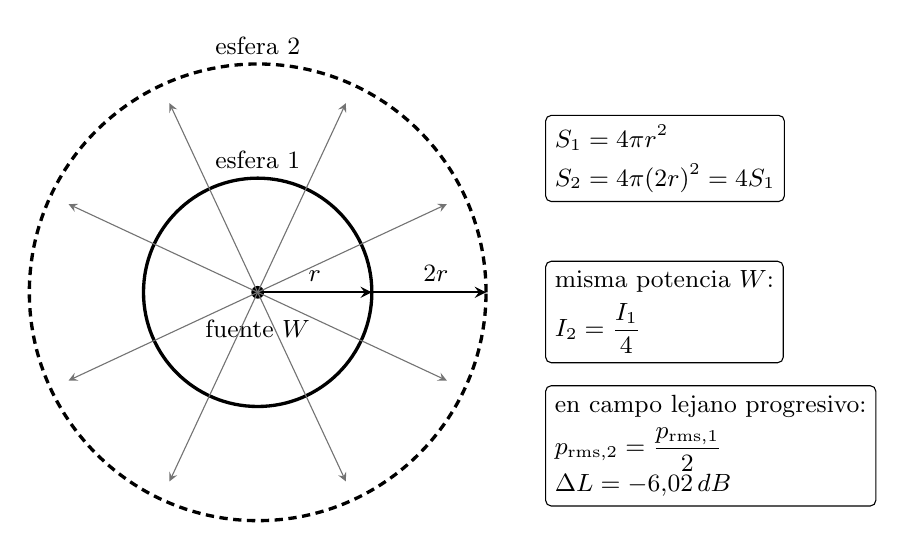
\begin{tikzpicture}[font=\small,>=stealth,x=1cm,y=1cm]
    \coordinate (S) at (3.35,3.20);
    \fill (S) circle (2.3pt);
    \node[below,fill=white,inner sep=1.5pt] at ([yshift=-3mm]S)
        {fuente \(W\)};

    \draw[very thick] (S) circle (1.45cm);
    \draw[very thick,densely dashed] (S) circle (2.90cm);
    \node[above] at (3.35,4.65) {esfera 1};
    \node[above] at (3.35,6.10) {esfera 2};

    \draw[->,thick] (S) -- (4.80,3.20)
        node[midway,above] {\(r\)};
    \draw[->,thick] (S) -- (6.25,3.20)
        node[pos=0.78,above] {\(2r\)};

    \foreach \a in {25,65,115,155,205,245,295,335}{
        \draw[->,black!55] (S) -- ++(\a:2.65);
    }

    \node[draw,rounded corners=2pt,align=left,anchor=west] at (7.00,4.90)
        {\(\displaystyle S_1=4\pi r^2\)\\[3pt]
         \(\displaystyle S_2=4\pi(2r)^2=4S_1\)};
    \node[draw,rounded corners=2pt,align=left,anchor=west] at (7.00,2.95)
        {misma potencia \(W\):\\[3pt]
         \(\displaystyle I_2=\frac{I_1}{4}\)};
    \node[draw,rounded corners=2pt,align=left,anchor=west] at (7.00,1.25)
        {en campo lejano progresivo:\\[3pt]
         \(\displaystyle p_{\mathrm{rms},2}
            =\frac{p_{\mathrm{rms},1}}{2}\)\\
         \(\displaystyle \Delta L=-6{,}02\,\text{dB}\)};
\end{tikzpicture}

    \caption{Propagación esférica ideal en sección. La misma potencia \(W\)
    atraviesa superficies de radios \(r\) y \(2r\); la segunda posee cuatro
    veces el área, por lo que \(I_2=I_1/4\). En campo lejano progresivo y con
    impedancia constante, \(p_{\mathrm{rms},2}=p_{\mathrm{rms},1}/2\).
    Elaboración propia a partir de las
    ecuaciones~\eqref{eq:u4-cuadrado-inverso}
    y~\eqref{eq:u4-razon-intensidades-distancia}; dibujo no a escala.}
    \label{fig:u4-propagacion-esferica}
\end{figure}

\subsection{Condiciones de validez}
\label{sec:u4-condiciones-cuadrado-inverso}

La ecuación~\eqref{eq:u4-nivel-presion-distancia} requiere:

\begin{itemize}
    \item una fuente suficientemente pequeña respecto de las distancias;
    \item comparación en una misma dirección de radiación;
    \item región de campo lejano;
    \item campo libre o reflexiones despreciables;
    \item propiedades aproximadamente uniformes del medio;
    \item absorción y otras pérdidas despreciables.
\end{itemize}

La Unidad~\ref{chap:unidad-9} aplicará este modelo a condiciones ambientales,
superficies y fuentes reales. Allí deberán considerarse las desviaciones
producidas por absorción, viento, gradientes de temperatura, suelo, obstáculos
y reflexiones.

\subsection{Ejemplo resuelto: nivel con la distancia}
\label{sec:u4-ejemplo-distancia}

Un nivel de presión sonora medido en campo libre es
\(L_{p1}=80\,\text{dB SPL}\) a \(r_1=1{,}0\,\text{m}\). Se desea estimar el
nivel a \(r_2=4{,}0\,\text{m}\), manteniendo las condiciones del modelo.

\[
    L_{p2}
      =80-20\log_{10}\!\left(\frac{4{,}0}{1{,}0}\right)
      \approx80-12{,}04
      \approx67{,}96\,\text{dB SPL}.
\]

Redondeado al decibel, el resultado es \(68\,\text{dB SPL}\). La disminución
se debe a la dispersión geométrica dentro del modelo; no incorpora absorción
atmosférica ni reflexiones.

\section{Omnidireccionalidad y directividad}
\label{sec:u4-directividad}

Una fuente \textbf{omnidireccional ideal} distribuye su potencia por igual en
todas las direcciones. Una fuente real puede radiar con distinta intensidad
según la dirección y la frecuencia.

Para describir esa concentración se define el \textbf{factor de directividad}
\(Q(\theta,\phi)\), adimensional, donde \(\theta\) y \(\phi\) indican una
dirección angular. En campo lejano, para una intensidad
\(I(r,\theta,\phi)\) medida a distancia \(r\) y una potencia total \(W\), el
factor puede expresarse como~\cite{xiangBlauert2021}

\begin{equation}
    Q(\theta,\phi)
      =\frac{I(r,\theta,\phi)}
             {W/(4\pi r^2)}.
    \label{eq:u4-factor-directividad}
\end{equation}

El denominador es la intensidad que tendría una fuente omnidireccional con la
misma potencia. En la dirección considerada, una fuente omnidireccional ideal
posee \(Q=1\).

El \textbf{índice de directividad} \(DI(\theta,\phi)\), medido en decibeles, se
define mediante

\begin{equation}
    DI(\theta,\phi)
      =10\log_{10}\!\left[Q(\theta,\phi)\right].
    \label{eq:u4-indice-directividad}
\end{equation}

Para \(Q=1\), \(DI=0\,\text{dB}\). Si en una dirección \(Q=4\),
\nopagebreak[4]

\[
    DI=10\log_{10}(4)\approx6{,}02\,\text{dB}.
\]

Esto significa que, a igual potencia total y distancia, el nivel asociado con
la intensidad en esa dirección supera en \(6{,}02\,\text{dB}\) al de la
fuente omnidireccional de comparación. No significa que la fuente haya creado
energía adicional.

La figura~\ref{fig:u4-directividad-q} compara secciones polares esquemáticas.
La forma del lóbulo direccional no representa un transductor particular:
solamente permite visualizar que \(Q\) es una comparación realizada a igual
potencia total y distancia.

\begin{figure}[htbp]
    \centering
    % Propósito: mostrar que la directividad redistribuye una potencia total sin
% crear energía y que Q compara intensidades a igual potencia y distancia.
% Origen: Q(theta,phi)=I(r,theta,phi)/(W/(4 pi r^2)), ecuación
% \eqref{eq:u4-factor-directividad}. Los patrones son esquemáticos y no
% corresponden a un transductor ni a una frecuencia medidos.
% Descripción accesible: a la izquierda, una sección polar circular representa
% una fuente omnidireccional. A la derecha, una sección con un lóbulo principal
% hacia la derecha representa una fuente direccional. En una dirección dada y
% a igual potencia y distancia, Q compara la intensidad direccional con la
% intensidad de la fuente omnidireccional.
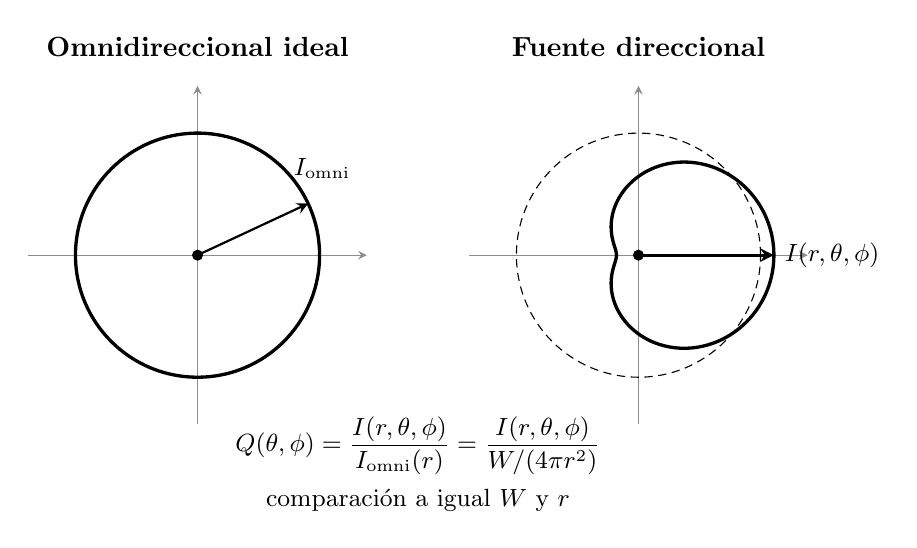
\begin{tikzpicture}[font=\small,>=stealth,x=1cm,y=1cm]
    \coordinate (O) at (2.95,2.75);
    \coordinate (D) at (8.55,2.75);

    \node[font=\bfseries] at (2.95,5.40) {Omnidireccional ideal};
    \node[font=\bfseries] at (8.55,5.40) {Fuente direccional};

    \draw[->,black!45] (0.80,2.75) -- (5.10,2.75);
    \draw[->,black!45] (2.95,0.60) -- (2.95,4.90);
    \draw[->,black!45] (6.40,2.75) -- (10.70,2.75);
    \draw[->,black!45] (8.55,0.60) -- (8.55,4.90);
    \fill (O) circle (2pt);
    \fill (D) circle (2pt);

    \draw[very thick] (O) circle (1.55cm);
    \node[anchor=west] at (4.05,3.85) {\(I_\mathrm{omni}\)};
    \draw[->,thick] (O) -- ++(25:1.55);

    \draw[very thick,samples=160,domain=0:360,smooth,variable=\a]
        plot ({8.55+(1.00+0.72*cos(\a))*cos(\a)},
              {2.75+(1.00+0.72*cos(\a))*sin(\a)});
    \draw[->,very thick] (D) -- ++(0:1.72)
        node[anchor=west] {\(I(r,\theta,\phi)\)};
    \draw[densely dashed] (D) circle (1.55cm);

    \node[align=center] at (5.75,0.10)
        {\(\displaystyle
          Q(\theta,\phi)
          =\frac{I(r,\theta,\phi)}
                 {I_\mathrm{omni}(r)}
          =\frac{I(r,\theta,\phi)}
                 {W/(4\pi r^2)}\)\\[4pt]
         comparación a igual \(W\) y \(r\)};
\end{tikzpicture}

    \caption{Comparación conceptual entre radiación omnidireccional y
    direccional. El factor \(Q(\theta,\phi)\) compara, a igual potencia total
    \(W\) y distancia \(r\), la intensidad en una dirección con la de una
    fuente omnidireccional ideal. Los patrones son esquemáticos y no codifican
    datos de un transductor. Elaboración propia a partir de la
    ecuación~\eqref{eq:u4-factor-directividad}.}
    \label{fig:u4-directividad-q}
\end{figure}

En el campo lejano, el modelo conjunto puede escribirse como

\begin{equation}
    I(r,\theta,\phi)
      =\frac{WQ(\theta,\phi)}{4\pi r^2}.
    \label{eq:u4-intensidad-directividad}
\end{equation}

La directividad depende de la frecuencia y de la geometría de la fuente. Su
aplicación en recintos y condiciones ambientales se reserva para el
Unidad~\ref{chap:unidad-9}.

\section{Relación con Fonoaudiología}
\label{sec:u4-fonoaudiologia}

Las magnitudes de esta unidad permiten interpretar qué informa un sistema de
medición y qué no puede inferirse sin datos adicionales.

\begin{itemize}
    \item Un micrófono calibrado responde a una variable acústica local. El
    instrumento puede procesar esa señal para informar un valor eficaz o un
    nivel de presión sonora.

    \item Un valor en \(\text{dB SPL}\) describe una relación física de
    presiones. No equivale por sí solo a sonoridad ni a un nivel en
    \(\text{dB HL}\).

    \item En audiometría, la interpretación del nivel presentado
    depende del transductor, de la frecuencia y de referencias de
    calibración~\cite{iso8253_1_2010,iso8253_2_2009}. Por esta razón, una presión medida en un punto no debe
    convertirse directamente en umbral audiométrico sin el procedimiento
    correspondiente.

    \item En una medición en campo sonoro, la distancia y la directividad
    importan, pero la ley del cuadrado inverso solo puede aplicarse cuando se
    cumplen sus hipótesis.

    \item La impedancia permite comprender por qué una interfaz puede producir
    reflexión y por qué presión y velocidad de partícula no conservan la misma
    relación en todos los campos.
\end{itemize}

Estas conexiones son introductorias. La anatomía y la mecánica del sistema
auditivo se desarrollarán más adelante, y los procedimientos clínicos no se
deducen únicamente de las ecuaciones acústicas de esta unidad.

\section{Errores frecuentes}
\label{sec:u4-errores}

\begin{description}[style=nextline]
    \item[\textbf{``La amplitud es el volumen o la intensidad''.}]
    La amplitud es el máximo valor de una magnitud oscilante y conserva su
    unidad. La intensidad se mide en \(\text{W}/\text{m}^2\); ``volumen'' no
    es el nombre de una magnitud acústica en este contexto.

    \item[\textbf{``Los decibeles miden intensidad''.}]
    El decibel expresa una relación. Debe indicarse si se trata de nivel de
    presión, intensidad, potencia, audición u otra magnitud.

    \item[\textbf{``Frecuencia y altura tonal son lo mismo''.}]
    La frecuencia es física y medible; la altura tonal es perceptual.

    \item[\textbf{``Dos fuentes iguales siempre agregan \(3\,\text{dB}\)''.}]
    El resultado depende de la correlación y, para fuentes coherentes, del
    desfase en el punto de observación.

    \item[\textbf{``Al duplicar la distancia, la intensidad cae
    \(6\,\text{dB}\)''.}]
    La intensidad se divide por cuatro. Su nivel y, bajo condiciones
    compatibles, el nivel de presión disminuyen aproximadamente
    \(6{,}02\,\text{dB}\).

    \item[\textbf{``Una cabina absorbente es un campo libre''.}]
    Un recinto real puede aproximar determinadas condiciones, pero requiere
    especificaciones y verificación.

    \item[\textbf{``Una onda en un tubo es cilíndrica''.}]
    La geometría del conducto no determina por sí sola la geometría del frente
    de onda.
\end{description}

\section{Síntesis}
\label{sec:u4-sintesis}

El sonido como fenómeno físico es una perturbación mecánica; la sensación
sonora es una respuesta perceptual. En un medio, la elasticidad y la inercia
permiten que la perturbación se propague mientras las partículas oscilan
localmente.

La presión acústica \(p\), la velocidad de partícula \(u\), la intensidad
\(I\), la potencia \(W\) y la energía \(E_\mathrm{ac}\) describen aspectos
diferentes del campo y poseen unidades diferentes. La impedancia relaciona
presión y velocidad bajo condiciones especificadas y ayuda a interpretar la
reflexión en una interfaz.

Una señal debe caracterizarse indicando si se usa un valor instantáneo, de
pico, pico a pico, medio o eficaz. El nivel de presión \(L_p\), el nivel de
intensidad \(L_I\) y el nivel de potencia \(L_W\) son relaciones logarítmicas;
no son sinónimos de sonoridad ni de nivel de audición.

Las presiones se suman instantáneamente. Para obtener un RMS o un nivel total
se debe conocer si las señales son coherentes, no correlacionadas o
parcialmente correlacionadas.

La onda plana, la cilíndrica y la esférica son modelos geométricos. La ley del
cuadrado inverso se deriva de la distribución de una potencia constante sobre
superficies esféricas y solo se aplica cuando se cumplen sus hipótesis. El
factor \(Q\) y el índice de directividad describen cómo cambia la radiación
con la dirección sin implicar creación de energía.

\section{Ejercicios de autoevaluación}
\label{sec:u4-ejercicios}

La secuencia comienza con distinciones conceptuales y lectura de figuras,
continúa con cálculos guiados y autónomos, y termina con aplicaciones,
integración y análisis de distractores. En los ejercicios numéricos se debe
escribir la ecuación utilizada, conservar las unidades durante el cálculo,
redondear solo el resultado final e interpretar su significado físico.

\subsection*{Preguntas conceptuales}

\begin{enumerate}[label=\textbf{C\arabic*.},leftmargin=*]
    \item Explique por qué un campo acústico puede existir aunque no haya un
    receptor presente.

    \item Describa qué funciones cumplen la elasticidad y la inercia del medio
    en la propagación. Indique por qué una onda sonora mecánica no se propaga
    en el vacío.

    \item Distinga velocidad de partícula y velocidad de propagación. Indique
    el símbolo y la unidad de cada una.

    \item Distinga presión acústica, intensidad y potencia mediante su
    significado físico y sus unidades.

    \item Una presión sinusoidal tiene valor medio cero. Explique por qué su
    valor eficaz puede ser distinto de cero.

    \item Indique por qué \(p/u=\rho c\) no debe aplicarse automáticamente a
    cualquier campo acústico.

    \item Distinga frecuencia y altura tonal. Distinga además nivel de presión
    sonora y sonoridad.

    \item Una medición se informa solamente como \(60\,\text{dB}\).
    ¿Qué información falta?
\end{enumerate}

\subsection*{Identificación e interpretación de gráficos}

\begin{enumerate}[label=\textbf{R\arabic*.},leftmargin=*]
    \item Observe la figura~\ref{fig:u4-impedancia-reflexion}.
    \begin{enumerate}[label=\alph*)]
        \item Identifique las ondas incidente, reflejada y transmitida, y
        describa el sentido de propagación de cada una.
        \item Si \(Z_{01}=Z_{02}\), indique el valor de \(R_p\) y cuál de las
        tres ondas desaparecería en el modelo ideal.
        \item Explique por qué la longitud de las flechas no permite leer las
        amplitudes de presión.
    \end{enumerate}

    \item Utilice la figura~\ref{fig:u4-presion-velocidad-intensidad}.
    \begin{enumerate}[label=\alph*)]
        \item Identifique qué curvas pueden tomar valores positivos y
        negativos y cuál permanece no negativa.
        \item Explique por qué \(i(t)=p(t)u(t)\) es positiva cuando \(p(t)\) y
        \(u(t)\) son simultáneamente negativas.
        \item La intensidad presenta dos máximos durante un período de
        presión. Explique por qué.
    \end{enumerate}

    \item Observe la figura~\ref{fig:u4-rms-sinusoide}.
    \begin{enumerate}[label=\alph*)]
        \item Explique cómo las áreas positivas y negativas justifican
        \(\overline p=0\,\text{Pa}\) durante un período.
        \item Lea el valor de
        \(\overline{p^2}/\hat p^{\,2}\).
        \item A partir de esa lectura, obtenga
        \(p_\mathrm{rms}/\hat p\).
    \end{enumerate}

    \item Utilice la figura~\ref{fig:u4-escala-presion-db-spl}.
    \begin{enumerate}[label=\alph*)]
        \item Compare \(p_\mathrm{rms}=0{,}020\,\text{Pa}\) y
        \(p_\mathrm{rms}=0{,}20\,\text{Pa}\): indique el factor de presión y
        el cambio de nivel.
        \item Compare \(p_\mathrm{rms}=2{,}0\,\text{mPa}\) y
        \(p_\mathrm{rms}=0{,}20\,\text{Pa}\).
        \item Explique por qué la figura no permite comparar sonoridades.
    \end{enumerate}

    \item Compare los dos paneles de la
    figura~\ref{fig:u4-suma-coherente-no-correlacionada}.
    \begin{enumerate}[label=\alph*)]
        \item Indique qué magnitud se duplica cuando dos presiones iguales y
        coherentes llegan en fase.
        \item Indique qué cantidades se suman cuando las señales no están
        correlacionadas.
        \item Explique por qué los aumentos son \(6{,}02\,\text{dB}\) y
        \(3{,}01\,\text{dB}\), respectivamente.
    \end{enumerate}

    \item Compare las figuras~\ref{fig:u4-propagacion-esferica}
    y~\ref{fig:u4-directividad-q}.
    \begin{enumerate}[label=\alph*)]
        \item Al pasar de \(r\) a \(2r\) en la primera figura, indique cómo
        cambian el área esférica, la intensidad, la presión eficaz y sus
        niveles bajo las condiciones declaradas.
        \item En la segunda figura, explique qué compara \(Q\) y por qué un
        lóbulo más concentrado no implica creación de potencia acústica.
    \end{enumerate}
\end{enumerate}

\subsection*{Ejercicios numéricos guiados}

\begin{enumerate}[label=\textbf{G\arabic*.},leftmargin=*]
    \item Una presión sinusoidal posee
    \(\hat p=0{,}141\,\text{Pa}\).
    \begin{enumerate}[label=\alph*)]
        \item Calcule \(p_\mathrm{pp}\).
        \item Calcule \(p_\mathrm{rms}\).
        \item Calcule \(L_p\) en aire usando
        \(p_\mathrm{ref}=20\,\mu\text{Pa}\).
    \end{enumerate}

    \item En una onda plana progresiva se adoptan
    \(p_\mathrm{rms}=0{,}100\,\text{Pa}\) y
    \(Z_0=4{,}00\times10^2\,\text{Pa}\,\text{s}/\text{m}\).
    La intensidad es uniforme y normal a una superficie
    \(S=0{,}500\,\text{m}^2\).
    \begin{enumerate}[label=\alph*)]
        \item Calcule \(u_\mathrm{rms}\).
        \item Calcule \(I\).
        \item Calcule la potencia \(W\) que atraviesa la superficie.
        \item Verifique las unidades de los tres resultados.
    \end{enumerate}

    \item En el modelo de campo libre se miden
    \(L_{p1}=70{,}0\,\text{dB SPL}\) a
    \(r_1=0{,}50\,\text{m}\). Estime el nivel a
    \(r_2=1{,}20\,\text{m}\) y enumere dos condiciones necesarias para usar
    la ecuación.
\end{enumerate}

\subsection*{Ejercicios numéricos autónomos}

\begin{enumerate}[label=\textbf{N\arabic*.},leftmargin=*]
    \item Para aire seco a
    \(\vartheta=15{,}0\,^{\circ}\text{C}\), utilice la aproximación de la
    ecuación~\eqref{eq:u2-velocidad-temperatura}. Calcule \(c\) y la longitud
    de onda de un tono de frecuencia \(f=500\,\text{Hz}\).

    \item Dos señales no correlacionadas producen niveles de
    \(L_1=70{,}0\,\text{dB SPL}\) y
    \(L_2=60{,}0\,\text{dB SPL}\) en el mismo punto. Calcule el nivel total.

    \item En un mismo punto se superponen dos tonos coherentes de igual presión
    eficaz. Cada uno produce por separado
    \(L_p=65{,}0\,\text{dB SPL}\), y la diferencia de fase es
    \(\Delta\varphi=\pi/2\,\text{rad}\). Calcule la presión eficaz resultante
    como múltiplo de la presión de uno de los tonos y el nivel resultante.

    \item Una interfaz ideal separa dos medios cuyas impedancias son
    \[
        Z_{01}=400\,\text{Pa}\,\text{s}/\text{m},
        \qquad
        Z_{02}=800\,\text{Pa}\,\text{s}/\text{m}.
    \]
    Calcule \(R_p\) y la fracción de intensidad reflejada \(R_I\).

    \item Una fuente presenta \(Q=8{,}0\) en una dirección. Calcule su índice
    de directividad.

    \item Una fuente puntual omnidireccional ideal emite
    \(W=0{,}0100\,\text{W}\). Calcule la intensidad a
    \(r=2{,}00\,\text{m}\) en campo libre.
\end{enumerate}

\subsection*{Aplicaciones en Fonoaudiología}

\begin{enumerate}[label=\textbf{F\arabic*.},leftmargin=*]
    \item Un informe contiene un umbral de \(35\,\text{dB HL}\) y otro valor de
    \(35\,\text{dB SPL}\). ¿Pueden considerarse iguales? Indique qué
    información adicional se necesitaría.

    \item En una medición mediante altavoz se registran
    \(72{,}0\,\text{dB SPL}\) a \(r_1=1{,}00\,\text{m}\). Se propone que a
    \(r_2=2{,}00\,\text{m}\) habrá exactamente
    \(66{,}0\,\text{dB SPL}\).
    \begin{enumerate}[label=\alph*)]
        \item Compruebe si el valor propuesto coincide con el modelo del
        cuadrado inverso.
        \item Explique por qué el resultado no queda garantizado en una sala
        o cabina real.
    \end{enumerate}

    \item Un micrófono informa
    \(L_p=80{,}0\,\text{dB SPL}\) en un punto. Explique qué describe ese dato y
    por qué no permite concluir por sí solo cuál fue la sonoridad percibida por
    una persona.
\end{enumerate}

\newpage
\subsection*{Pregunta integradora}

\begin{enumerate}[label=\textbf{I\arabic*.},leftmargin=*]
    \item Se propone un modelo didáctico sin presencia de oyentes. Una fuente
    emite una potencia acústica constante
    \(W=0{,}0200\,\text{W}\) y posee
    \(Q=4{,}00\) en la dirección considerada. En campo libre y campo lejano,
    el medio tiene
    \(Z_0=4{,}00\times10^2\,\text{Pa}\,\text{s}/\text{m}\). Se adopta para el aire
    \(p_\mathrm{ref}=20\,\mu\text{Pa}\).
    \begin{enumerate}[label=\alph*)]
        \item Calcule la intensidad \(I_1\) a
        \(r_1=2{,}00\,\text{m}\).
        \item Calcule \(p_{\mathrm{rms},1}\) mediante la relación de onda
        progresiva.
        \item Calcule \(L_{p1}\).
        \item Repita los tres resultados para
        \(r_2=4{,}00\,\text{m}\), en la misma dirección.
        \item Explique por qué \(Q\) no crea potencia adicional y por qué
        ninguno de los niveles calculados determina una sonoridad única.
    \end{enumerate}
\end{enumerate}

\subsection*{Errores frecuentes y distractores}

En cada caso, determine si la respuesta propuesta es correcta. Si no lo es,
identifique el distractor y escriba la corrección.

\begin{enumerate}[label=\textbf{D\arabic*.},leftmargin=*]
    \item Para una presión sinusoidal de media nula se propone
    \(p_\mathrm{rms}=0\,\text{Pa}\) y, por lo tanto, ausencia de transferencia
    media de energía.

    \item Como \(p/u=\rho c\), se propone usar esta relación en cualquier
    punto de un campo estacionario o reverberante.

    \item Dos señales no correlacionadas producen por separado
    \(60{,}0\,\text{dB SPL}\). Se propone que juntas producen
    \(120\,\text{dB SPL}\).

    \item Para una fuente puntual omnidireccional ideal, al pasar de
    \(r_1=1{,}00\,\text{m}\) a \(r_2=2{,}00\,\text{m}\) se propone que la
    intensidad se divide por dos y la presión eficaz por cuatro.

    \item Se propone que \(50\,\text{dB SPL}\) y
    \(50\,\text{dB HL}\) describen necesariamente el mismo estímulo físico
    porque poseen el mismo valor numérico.

    \item Para una fuente con \(Q=4{,}0\) se propone que su potencia total es
    cuatro veces mayor que la potencia de la fuente omnidireccional usada como
    comparación.

    \item Una potencia aumenta de \(W_1=1{,}0\,\text{mW}\) a
    \(W_2=2{,}0\,\text{mW}\). Se propone un aumento de
    \(20\log_{10}(2)=6{,}02\,\text{dB}\).
\end{enumerate}

\section{Soluciones de los ejercicios}
\label{sec:u4-soluciones}

\subsection*{Preguntas conceptuales}

\begin{enumerate}[label=\textbf{C\arabic*.},leftmargin=*]
    \item El campo físico es una propiedad del medio perturbado. Un receptor
    permite detectarlo, pero no es necesario para que la perturbación exista.

    \item La elasticidad produce una acción restauradora después de una
    compresión o rarefacción; la inercia hace que el movimiento local no cambie
    instantáneamente. La interacción entre regiones vecinas permite la
    propagación. En el vacío no existe un medio material que pueda sostener
    esa interacción mecánica.

    \item La velocidad de partícula \(\mathbf u\) describe el movimiento local
    y puede cambiar de sentido durante un ciclo. La velocidad de propagación
    \(c\) describe el avance de un estado de la onda. Ambas se miden en
    \(\text{m}/\text{s}\), pero no son la misma magnitud.

    \item La presión acústica \(p\) es una variación local de presión y se mide
    en \(\text{Pa}\). La intensidad \(I\) es flujo medio de energía por área y
    se mide en \(\text{W}/\text{m}^2\). La potencia \(W\) es energía
    transferida por unidad de tiempo y se mide en \(\text{W}\).

    \item Las partes positivas y negativas se cancelan en el valor medio. En
    el cálculo eficaz se eleva primero la presión al cuadrado, por lo que esas
    contribuciones no se cancelan, y luego se toma la raíz cuadrada.

    \item La relación supone una onda plana progresiva en un medio homogéneo y
    sin pérdidas. En campos estacionarios, próximos o reverberantes, presión y
    velocidad pueden presentar otra relación de amplitud y fase.

    \item La frecuencia y el nivel de presión sonora son magnitudes físicas.
    La altura tonal y la sonoridad son atributos perceptuales que también
    dependen de otras propiedades de la señal, del oyente y del contexto.

    \item Se debe indicar qué nivel es, cuál es su referencia y si posee una
    ponderación u otra condición adicional.
\end{enumerate}

\subsection*{Identificación e interpretación de gráficos}

\begin{enumerate}[label=\textbf{R\arabic*.},leftmargin=*]
    \item
    \begin{enumerate}[label=\alph*)]
        \item La onda incidente avanza hacia la interfaz; la reflejada regresa
        por el primer medio y la transmitida se aleja de la interfaz por el
        segundo medio.
        \item Si \(Z_{01}=Z_{02}\), entonces \(R_p=0\) y desaparece la onda
        reflejada en el modelo ideal.
        \item Las flechas codifican dirección y tipo de onda. El epígrafe
        aclara que el esquema no representa proporciones de amplitud.
    \end{enumerate}

    \item
    \begin{enumerate}[label=\alph*)]
        \item \(p(t)\) y \(u(t)\) toman valores positivos y negativos;
        \(i(t)\) permanece no negativa en el caso representado.
        \item Cuando \(p(t)<0\,\text{Pa}\) y
        \(u(t)<0\,\text{m}/\text{s}\), su producto es positivo y conserva la
        unidad \(\text{W}/\text{m}^2\).
        \item Como las dos sinusoides están en fase,
        \[
            i(t)\propto\sin^2(2\pi ft+\varphi).
        \]
        Esta función alcanza dos máximos durante un período de \(p(t)\).
    \end{enumerate}

    \item
    \begin{enumerate}[label=\alph*)]
        \item Durante un período completo, las contribuciones positivas y
        negativas de \(p(t)\) tienen igual área algebraica y
        \(\overline p=0\,\text{Pa}\).
        \item La figura indica
        \(\overline{p^2}/\hat p^{\,2}=1/2\).
        \item
        \[
            \frac{p_\mathrm{rms}}{\hat p}
              =\sqrt{\frac{1}{2}}
              =\frac{1}{\sqrt{2}}.
        \]
    \end{enumerate}

    \item
    \begin{enumerate}[label=\alph*)]
        \item La presión se multiplica por \(10\) y el nivel aumenta
        \(20\,\text{dB}\): pasa de \(60\,\text{dB SPL}\) a
        \(80\,\text{dB SPL}\).
        \item \(0{,}20\,\text{Pa}=200\,\text{mPa}\), por lo que la presión es
        \(100\) veces mayor que \(2{,}0\,\text{mPa}\). El nivel pasa de
        \(40\,\text{dB SPL}\) a \(80\,\text{dB SPL}\), un aumento de
        \(40\,\text{dB}\).
        \item La escala representa una relación matemática entre presión
        eficaz y nivel; no incorpora frecuencia, duración, espectro, oyente ni
        contexto perceptual.
    \end{enumerate}

    \item
    \begin{enumerate}[label=\alph*)]
        \item En el caso coherente y en fase se duplica la presión resultante.
        \item En el caso no correlacionado se suman los cuadrados de las
        presiones eficaces.
        \item Duplicar la presión produce
        \(20\log_{10}(2)=6{,}02\,\text{dB}\). Duplicar la suma cuadrática
        produce \(10\log_{10}(2)=3{,}01\,\text{dB}\).
    \end{enumerate}

    \item
    \begin{enumerate}[label=\alph*)]
        \item Al duplicar el radio, el área se cuadruplica, la intensidad se
        divide por cuatro y la presión eficaz se divide por dos. El nivel de
        intensidad y el de presión disminuyen
        \(6{,}02\,\text{dB}\) bajo las condiciones indicadas.
        \item \(Q\) compara intensidades en una dirección, a igual potencia
        total y distancia. La directividad redistribuye la potencia entre
        direcciones; no aumenta la potencia total.
    \end{enumerate}
\end{enumerate}

\subsection*{Ejercicios numéricos guiados}

\begin{enumerate}[label=\textbf{G\arabic*.},leftmargin=*]
    \item
    \begin{enumerate}[label=\alph*)]
        \item \(p_\mathrm{pp}=2(0{,}141\,\text{Pa})
        =0{,}282\,\text{Pa}\).
        \item \(p_\mathrm{rms}
        =0{,}141/\sqrt{2}\,\text{Pa}
        \approx0{,}0997\,\text{Pa}\).
        \item
        \[
            L_p
              =20\log_{10}\!\left(
               \frac{0{,}0997}
                    {2{,}0\times10^{-5}}\right)
              \approx74{,}0\,\text{dB SPL}.
        \]
    \end{enumerate}

    \item
    \begin{enumerate}[label=\alph*)]
        \item
        \[
            u_\mathrm{rms}
              =\frac{0{,}100\,\text{Pa}}
                     {4{,}00\times10^2\,
                      \text{Pa}\,\text{s}/\text{m}}
              =2{,}50\times10^{-4}\,\text{m}/\text{s}.
        \]
        \item
        \[
            I=\frac{(0{,}100\,\text{Pa})^2}
                    {4{,}00\times10^2\,
                     \text{Pa}\,\text{s}/\text{m}}
             =2{,}50\times10^{-5}\,\text{W}/\text{m}^2.
        \]
        \item
        \[
            W=IS
             =(2{,}50\times10^{-5}\,\text{W}/\text{m}^2)
              (0{,}500\,\text{m}^2)
             =1{,}25\times10^{-5}\,\text{W}.
        \]
        \item El cociente
        \(\text{Pa}/(\text{Pa}\,\text{s}/\text{m})\) produce
        \(\text{m}/\text{s}\). El cociente
        \(\text{Pa}^2/(\text{Pa}\,\text{s}/\text{m})\) produce
        \(\text{W}/\text{m}^2\), y
        \((\text{W}/\text{m}^2)\text{m}^2=\text{W}\).
    \end{enumerate}

    \item
    \[
        L_{p2}
          =70{,}0-20\log_{10}\!\left(
             \frac{1{,}20}{0{,}50}\right)
          \approx62{,}40\,\text{dB SPL}.
    \]
    Con la precisión de los datos, se informa
    \(L_{p2}\approx62{,}4\,\text{dB SPL}\).
    Entre las condiciones posibles se encuentran campo libre, campo lejano,
    misma dirección de radiación, fuente suficientemente pequeña, medio
    uniforme y pérdidas despreciables.
\end{enumerate}

\subsection*{Ejercicios numéricos autónomos}

\begin{enumerate}[label=\textbf{N\arabic*.},leftmargin=*]
    \item
    \[
        c\approx331+0{,}6(15{,}0)
          =340\,\text{m}/\text{s},
        \qquad
        \lambda=\frac{c}{f}
          =\frac{340\,\text{m}/\text{s}}{500\,\text{Hz}}
          =0{,}680\,\text{m}.
    \]

    \item
    \[
        L_\mathrm{R}
          =10\log_{10}\!\left(10^7+10^6\right)
          =10\log_{10}(1{,}1\times10^7)
          \approx70{,}4\,\text{dB SPL}.
    \]

    \item Para presiones eficaces iguales \(p\),
    \[
        p_\mathrm{R,rms}^2
          =p^2+p^2+2p^2\cos(\pi/2)
          =2p^2,
        \qquad
        p_\mathrm{R,rms}=\sqrt{2}\,p.
    \]
    Por lo tanto,
    \[
        L_\mathrm{R}
          =65{,}0+20\log_{10}(\sqrt{2})
          \approx68{,}0\,\text{dB SPL}.
    \]
    El aumento coincide numéricamente con \(3{,}01\,\text{dB}\), pero aquí
    resulta de un desfase coherente de \(\pi/2\,\text{rad}\), no de falta de
    correlación.

    \item
    \[
        R_p=\frac{800-400}{800+400}=\frac{1}{3},
        \qquad
        R_I=\left(\frac{1}{3}\right)^2=\frac{1}{9}\approx0{,}111.
    \]
    El modelo predice una reflexión del \(11{,}1\%\) de la intensidad
    incidente bajo las condiciones declaradas.

    \item
    \[
        DI=10\log_{10}(8{,}0)\approx9{,}0\,\text{dB}.
    \]

    \item
    \[
        I=\frac{0{,}0100\,\text{W}}
                {4\pi(2{,}00\,\text{m})^2}
          \approx1{,}99\times10^{-4}\,\text{W}/\text{m}^2.
    \]
\end{enumerate}

\subsection*{Aplicaciones en Fonoaudiología}

\begin{enumerate}[label=\textbf{F\arabic*.},leftmargin=*]
    \item No. El valor en \(\text{dB HL}\) depende de referencias
    audiométricas relacionadas con la frecuencia y el transductor. Se
    necesitarían, como mínimo, la frecuencia, el transductor y los datos de
    calibración correspondientes.

    \item
    \begin{enumerate}[label=\alph*)]
        \item
        \[
            L_{p2}
              =72{,}0-20\log_{10}\!\left(
                 \frac{2{,}00}{1{,}00}\right)
              \approx66{,}0\,\text{dB SPL}.
        \]
        El valor propuesto coincide, dentro del redondeo, con el modelo ideal.
        \item En una sala o cabina pueden existir reflexiones, campo próximo,
        directividad, absorción y otras desviaciones. También deben mantenerse
        la misma dirección de radiación y condiciones comparables de
        medición.
    \end{enumerate}

    \item El dato expresa una relación entre la presión eficaz medida y la
    referencia de \(20\,\mu\text{Pa}\) usada en aire. La sonoridad depende
    además de frecuencia, duración, contenido espectral, contexto y
    características del oyente; por eso el nivel físico no determina una
    respuesta perceptual única.
\end{enumerate}

\subsection*{Pregunta integradora}

\begin{enumerate}[label=\textbf{I\arabic*.},leftmargin=*]
    \item
    \begin{enumerate}[label=\alph*)]
        \item
        \[
            I_1
              =\frac{WQ}{4\pi r_1^2}
              =\frac{(0{,}0200\,\text{W})(4{,}00)}
                     {4\pi(2{,}00\,\text{m})^2}
              \approx1{,}59\times10^{-3}\,\text{W}/\text{m}^2.
        \]
        \item
        \[
            I_1Z_0
              \approx
              (1{,}59\times10^{-3}\,\text{W}/\text{m}^2)
              (4{,}00\times10^2\,
               \text{Pa}\,\text{s}/\text{m})
              \approx0{,}637\,\text{Pa}^2,
        \]
        \[
            p_{\mathrm{rms},1}
              =\sqrt{I_1Z_0}
              \approx\sqrt{0{,}637\,\text{Pa}^2}
              \approx0{,}798\,\text{Pa}.
        \]
        \item
        \[
            L_{p1}
              =20\log_{10}\!\left(
                \frac{0{,}798\,\text{Pa}}
                     {20\times10^{-6}\,\text{Pa}}\right)
              \approx92{,}0\,\text{dB SPL}.
        \]
        \item Al duplicar la distancia,
        \[
            I_2=\frac{I_1}{4}
              \approx3{,}98\times10^{-4}\,\text{W}/\text{m}^2,
            \qquad
            p_{\mathrm{rms},2}=\frac{p_{\mathrm{rms},1}}{2}
              \approx0{,}399\,\text{Pa},
        \]
        \[
            L_{p2}
              =L_{p1}-20\log_{10}(2)
              \approx86{,}0\,\text{dB SPL}.
        \]
        \item \(Q\) redistribuye la potencia total entre direcciones; no la
        crea. Los niveles calculados describen relaciones físicas de presión,
        pero la sonoridad depende además de otras propiedades del estímulo y
        del oyente.
    \end{enumerate}
\end{enumerate}

\subsection*{Errores frecuentes y distractores}

\begin{enumerate}[label=\textbf{D\arabic*.},leftmargin=*]
    \item La propuesta es incorrecta. Para una sinusoide de media nula,
    \(p_\mathrm{rms}=\hat p/\sqrt{2}\), no cero. En una onda progresiva,
    presión y velocidad pueden producir una intensidad media no nula.

    \item La propuesta es incorrecta. La relación
    \(p/u=\rho c\) utilizada en esta unidad requiere una onda plana progresiva,
    un medio homogéneo y el modelo sin pérdidas; no se traslada
    automáticamente a campos estacionarios o reverberantes.

    \item La propuesta es incorrecta. Para dos señales no correlacionadas de
    igual nivel,
    \[
        L_\mathrm{R}
          =60{,}0+10\log_{10}(2)
          \approx63{,}0\,\text{dB SPL}.
    \]
    Los valores expresados en decibeles no se suman directamente.

    \item La propuesta es incorrecta. En el modelo esférico ideal,
    \(I_2=I_1/4\) y
    \(p_{\mathrm{rms},2}=p_{\mathrm{rms},1}/2\). Ambos niveles disminuyen
    \(6{,}02\,\text{dB}\) bajo las condiciones declaradas.

    \item La propuesta es incorrecta. \(\text{dB SPL}\) usa una referencia
    física de presión; \(\text{dB HL}\) usa referencias audiométricas que
    dependen, entre otros factores, de la frecuencia y del transductor.

    \item La propuesta es incorrecta. \(Q=4{,}0\) indica que, en la dirección
    considerada y a igual distancia, la intensidad es cuatro veces la de una
    fuente omnidireccional de igual potencia total. La potencia no aumenta.

    \item La propuesta es incorrecta. Para una razón de potencias se utiliza
    el factor \(10\):
    \[
        L_{W2}-L_{W1}
          =10\log_{10}\!\left(
            \frac{2{,}0\,\text{mW}}{1{,}0\,\text{mW}}\right)
          \approx3{,}01\,\text{dB}.
    \]
\end{enumerate}

\section{Glosario}
\label{sec:u4-glosario}

\begin{description}[nosep]
    \item[\textbf{Campo acústico:}] distribución espacial y temporal de
    magnitudes como presión, velocidad de partícula e intensidad.
    \item[\textbf{Coherencia:}] relación temporal estable entre señales; para
    sinusoides de igual frecuencia implica una diferencia de fase constante.
    \item[\textbf{Factor de directividad (\(Q\)):}] razón adimensional entre
    la intensidad en una dirección y la intensidad de una fuente
    omnidireccional de igual potencia y distancia.
    \item[\textbf{Impedancia acústica específica (\(Z\)):}] relación entre
    presión acústica y velocidad de partícula bajo condiciones especificadas;
    se mide en \(\text{Pa}\,\text{s}/\text{m}\).
    \item[\textbf{Índice de directividad (\(DI\)):}] expresión logarítmica del
    factor de directividad; se mide en decibeles.
    \item[\textbf{Intensidad acústica (\(I\)):}] flujo medio de energía
    acústica por unidad de área; se mide en \(\text{W}/\text{m}^2\).
    \item[\textbf{Nivel de presión sonora (\(L_p\)):}] relación logarítmica
    entre una presión eficaz y una presión de referencia.
    \item[\textbf{Potencia acústica (\(W\)):}] energía acústica transferida por
    unidad de tiempo; se mide en watts (\(\text{W}\)).
    \item[\textbf{Presión acústica (\(p\)):}] variación de presión respecto de
    la presión estática local; se mide en pascales (\(\text{Pa}\)).
    \item[\textbf{Valor eficaz o RMS:}] raíz cuadrada del promedio del cuadrado
    de una señal durante un intervalo especificado.
    \item[\textbf{Velocidad de partícula (\(\mathbf u\)):}] velocidad local de
    una pequeña región del medio; se mide en \(\text{m}/\text{s}\).
\end{description}

%%%%%%%%%%%%%%%%%%%%%%%%%%%%%%%%%%%%%%%%%%%%%%%%%%%%%%%%%%%%%%%%%%%%%%%%%%%%%%%%%%%%%%%%%%%%%%%%%%
